% !TeX root = main.tex
\section{Mask design}
\begin{figure}[H]
    \centering
    
\includegraphics[trim=0mm 0.12mm 0.17mm 0mm, clip=true,width=\linewidth]{figures/litho_design.pdf}
    \captionof{figure}{Used lithography design}
    \label{fig:litho_design}
\end{figure}

The design for the mask was made to enable easy detection of the attained resolution with certain patterns. This was done by taking patterns specifically designed to test the resolution and/or by taking patterns that are common in the semiconductor industry.

Starting from the top left and moving clockwise,

\begin{itemize}
    \item Checkerboard
    \item Single line surround by multiple lines
    \item Outward radiating lines
    \item Internally touching circles
    \item Shapes with OPC
    \item Slightly non-parallel lines
    \item Koch snowflake
\end{itemize}

The checkerboard pattern is a widely used pattern in micro- and nanofabrication checkerboard pattern, allowing easy detection of over- and underexposure. The next pattern is a much seen pattern in nanofabrication, and is important for analyzing the effect of interference when multiple lines are close together. The outward radiating lines have the feature that the distance between the lines becomes smaller towards the center, making it possible to see at what length scale the lines are still separable. This principle also holds for the internally touching circles. In the top right there is a square with an (approximate) optical proximity correction (OPC) pattern. The Koch snowflake has (in the idealized case) infinite detail, allowing the comparison between the different length scales of the snowflake to see where the resolution becomes too low to see the details. Note that this version has only five iterations, since infinite detail would be unpractical.

\section{Inspection images}\label{ap:inspec_img}
% \todo[inline]{ik krijg de titel niet op dezelfde pagina als de plaatjes..}
% % \todo[inline]{Optical microscope images of mask}
% \begin{figure*}[!t]	
%     \centering
%     \begin{subfigure}[t]{0.24\linewidth}
%     	\centering
%  	\resizebox{\linewidth}{!}{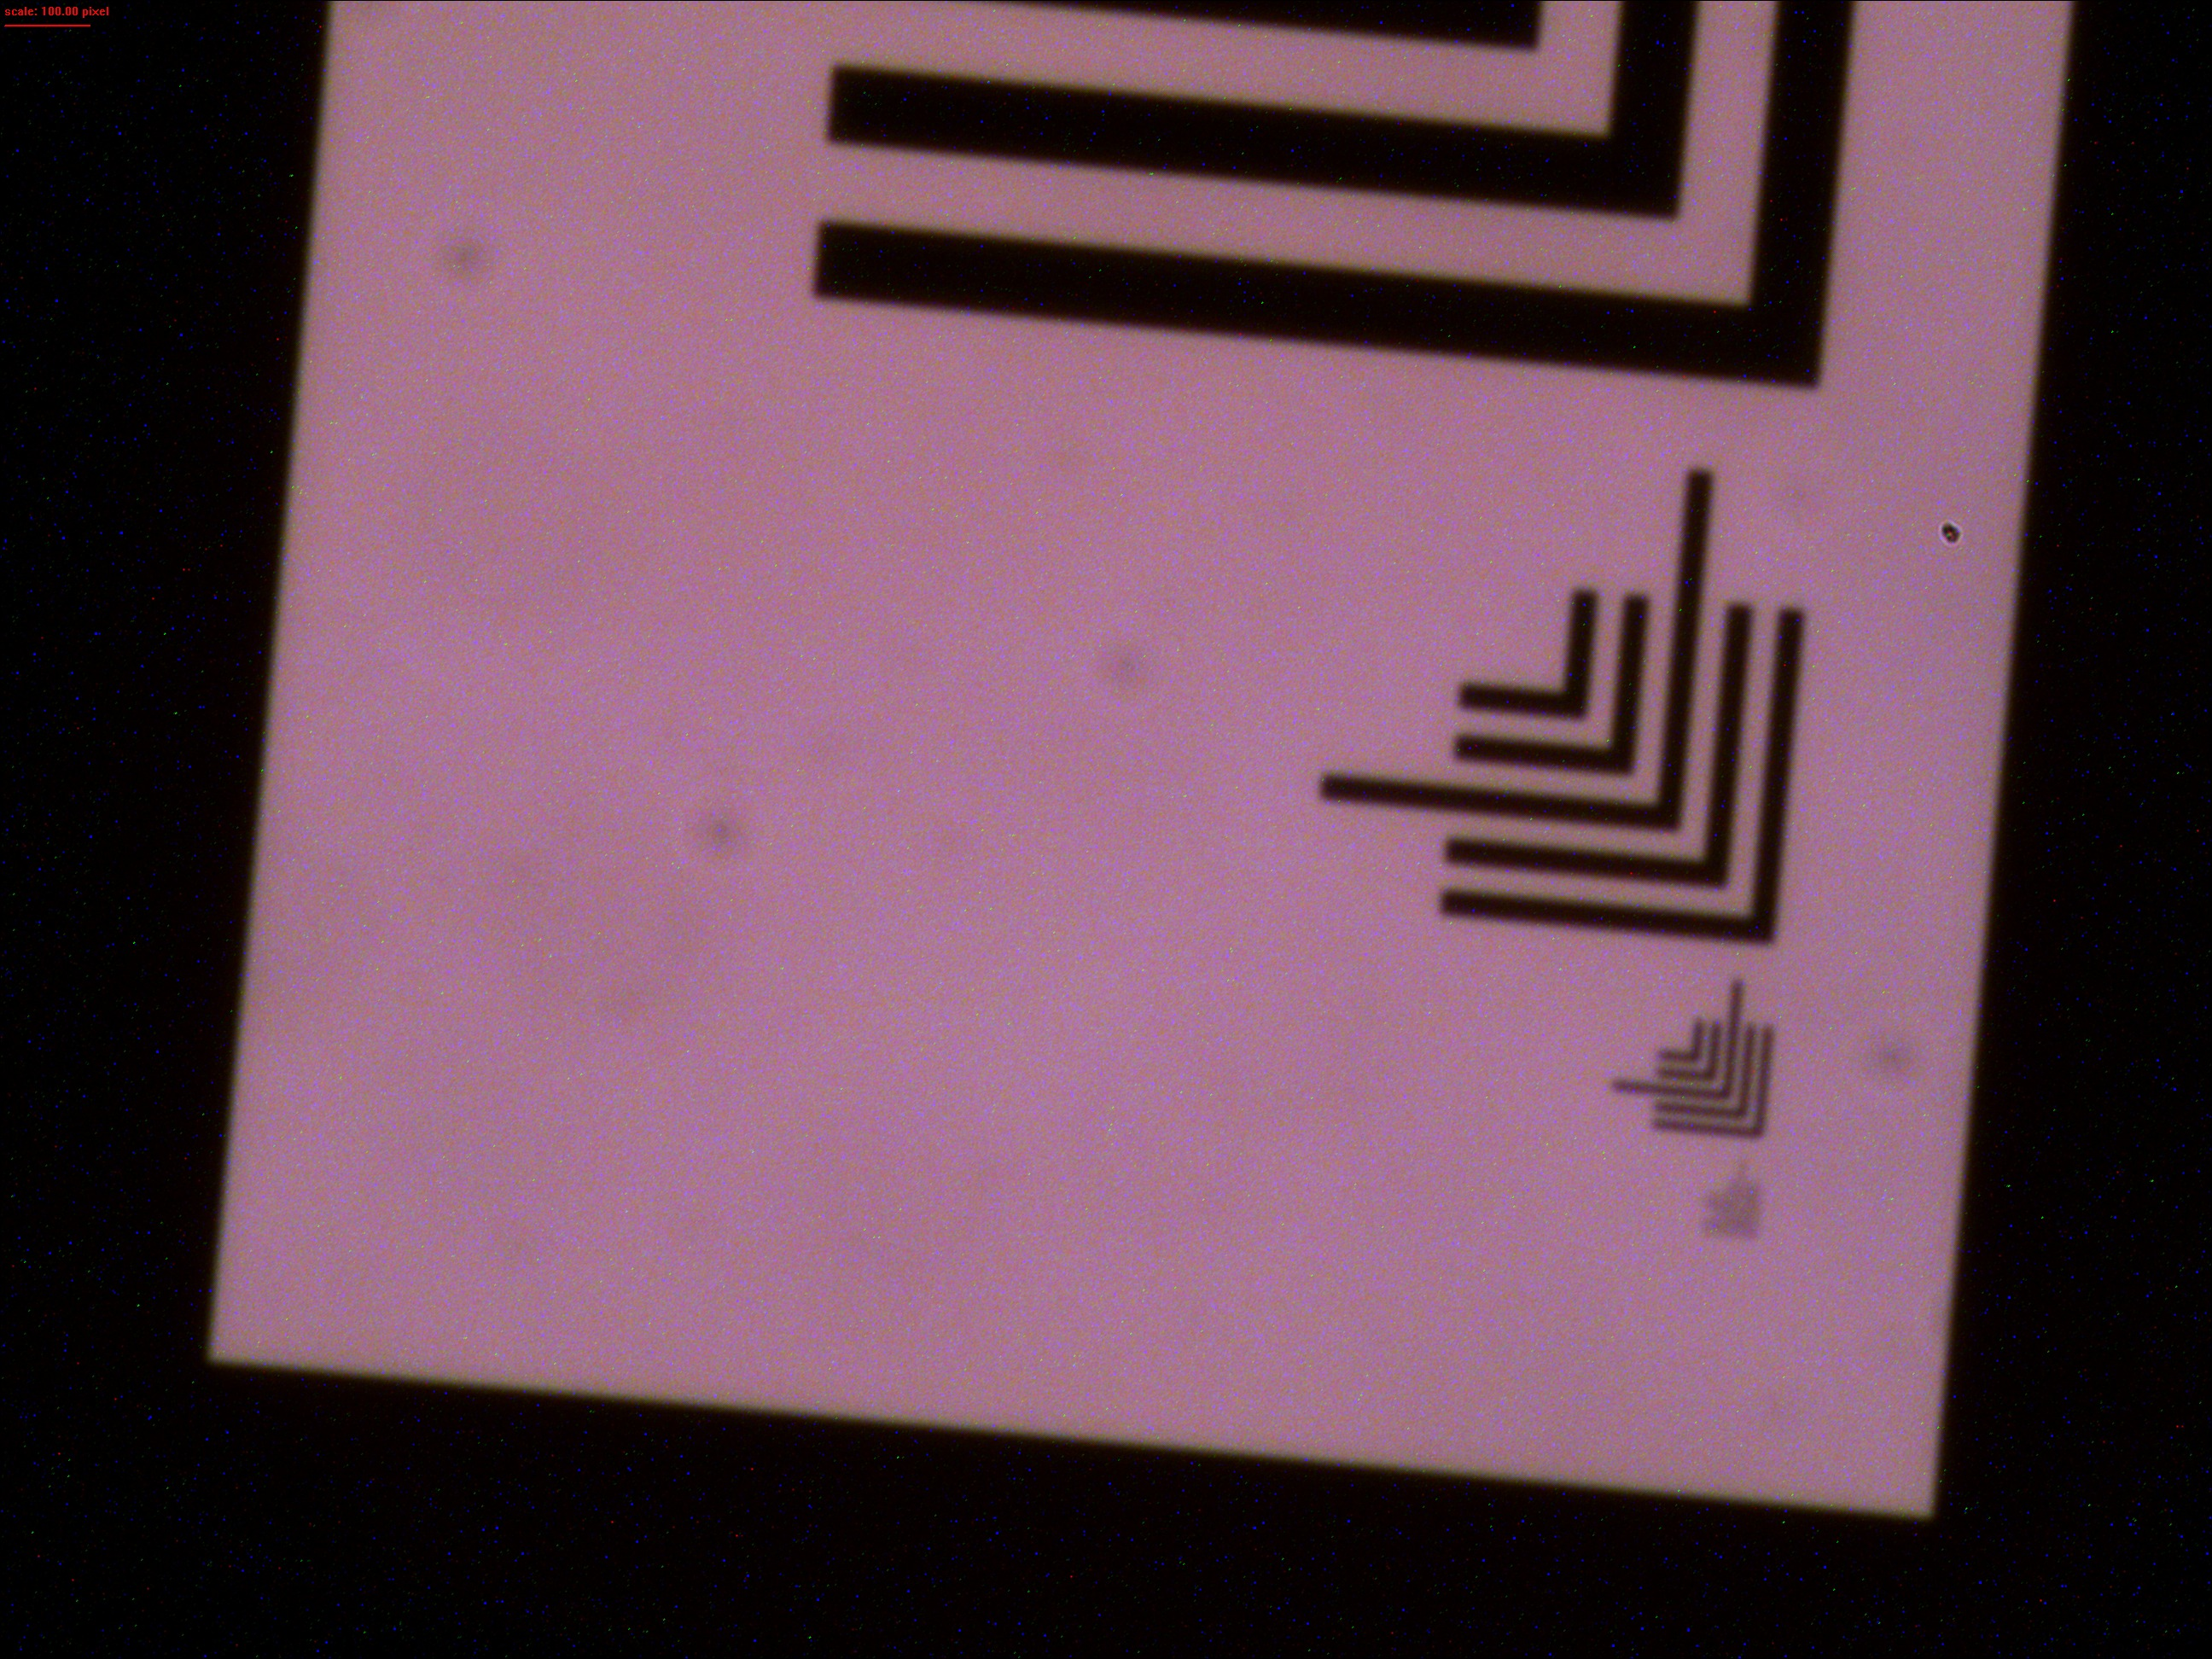
\includegraphics{data/mask/TS_05_20_13_50_44.jpg}}
%  	\caption{Mask}
%  	\label{fig:TS_05_20_13_50_44}
%  \end{subfigure}
%     \hfill
%     \begin{subfigure}[t]{0.24\linewidth}
%  	\centering
%  	\resizebox{\linewidth}{!}{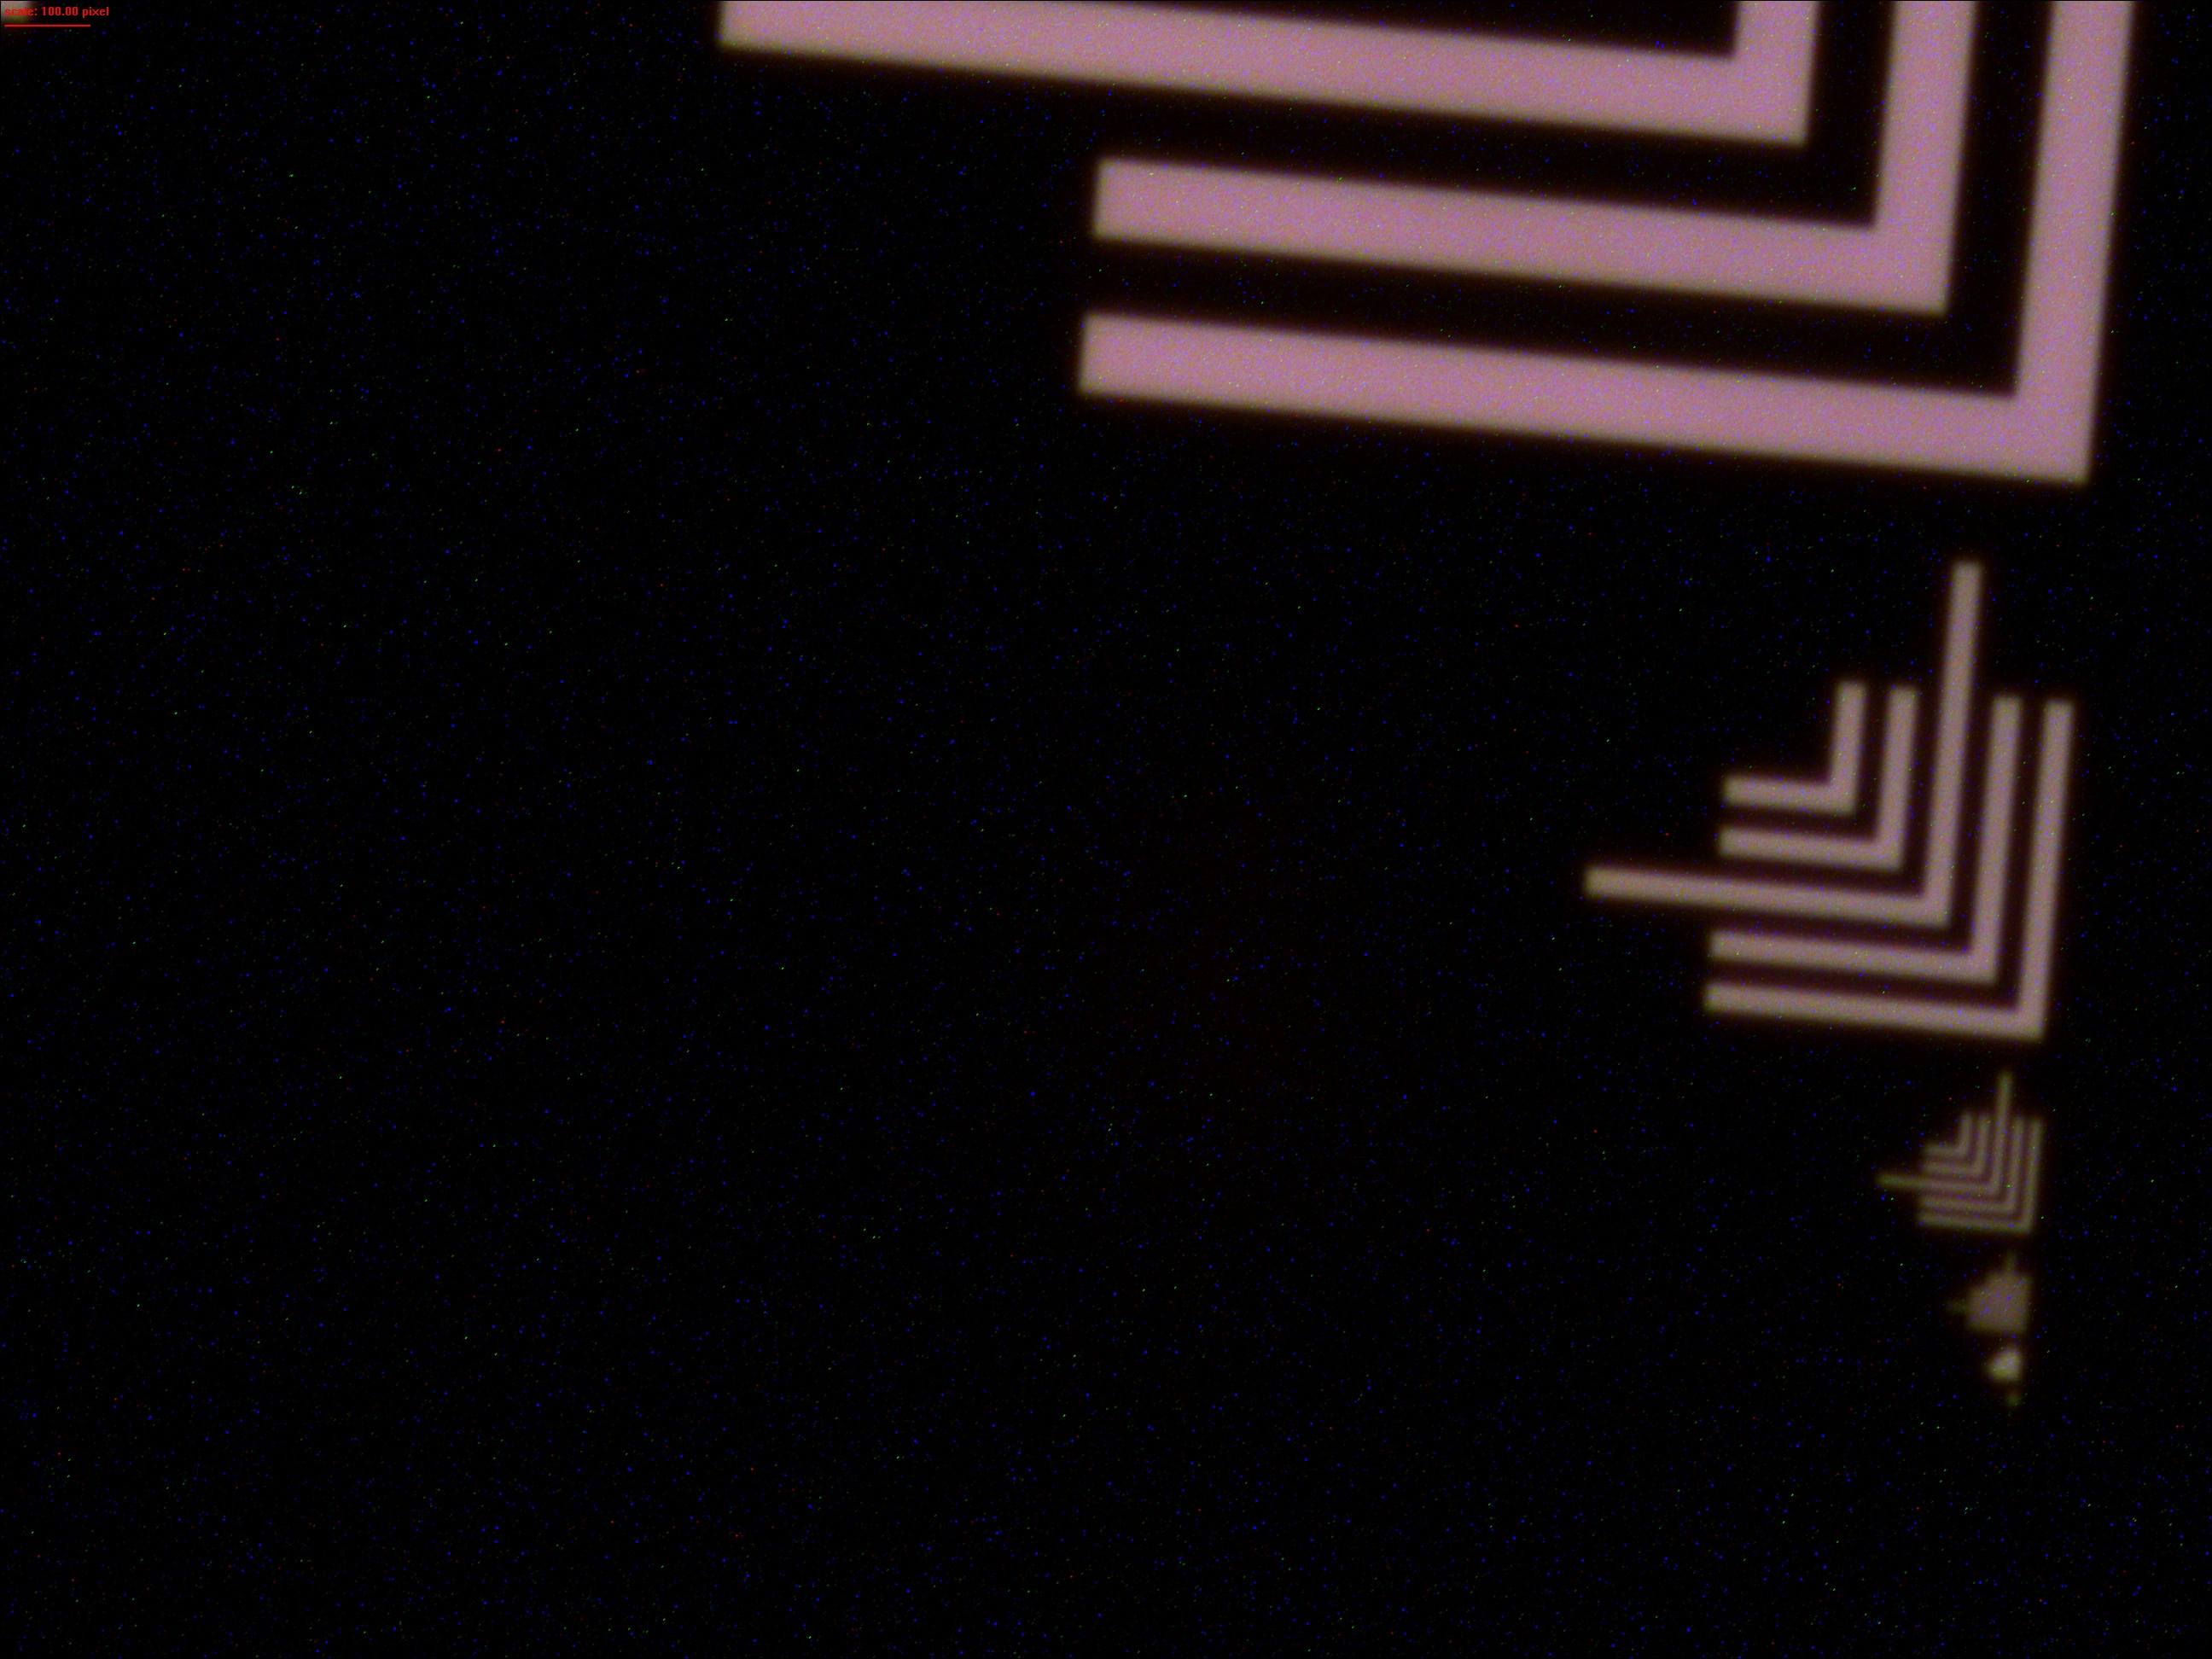
\includegraphics{data/mask/TS_05_20_13_51_16.jpg}}
%  	\caption{Mask}
%  	\label{fig:TS_05_20_13_51_16}
%  \end{subfigure}
%     \hfill
%     \begin{subfigure}[t]{0.24\linewidth}
%  	\centering
%  	\resizebox{\linewidth}{!}{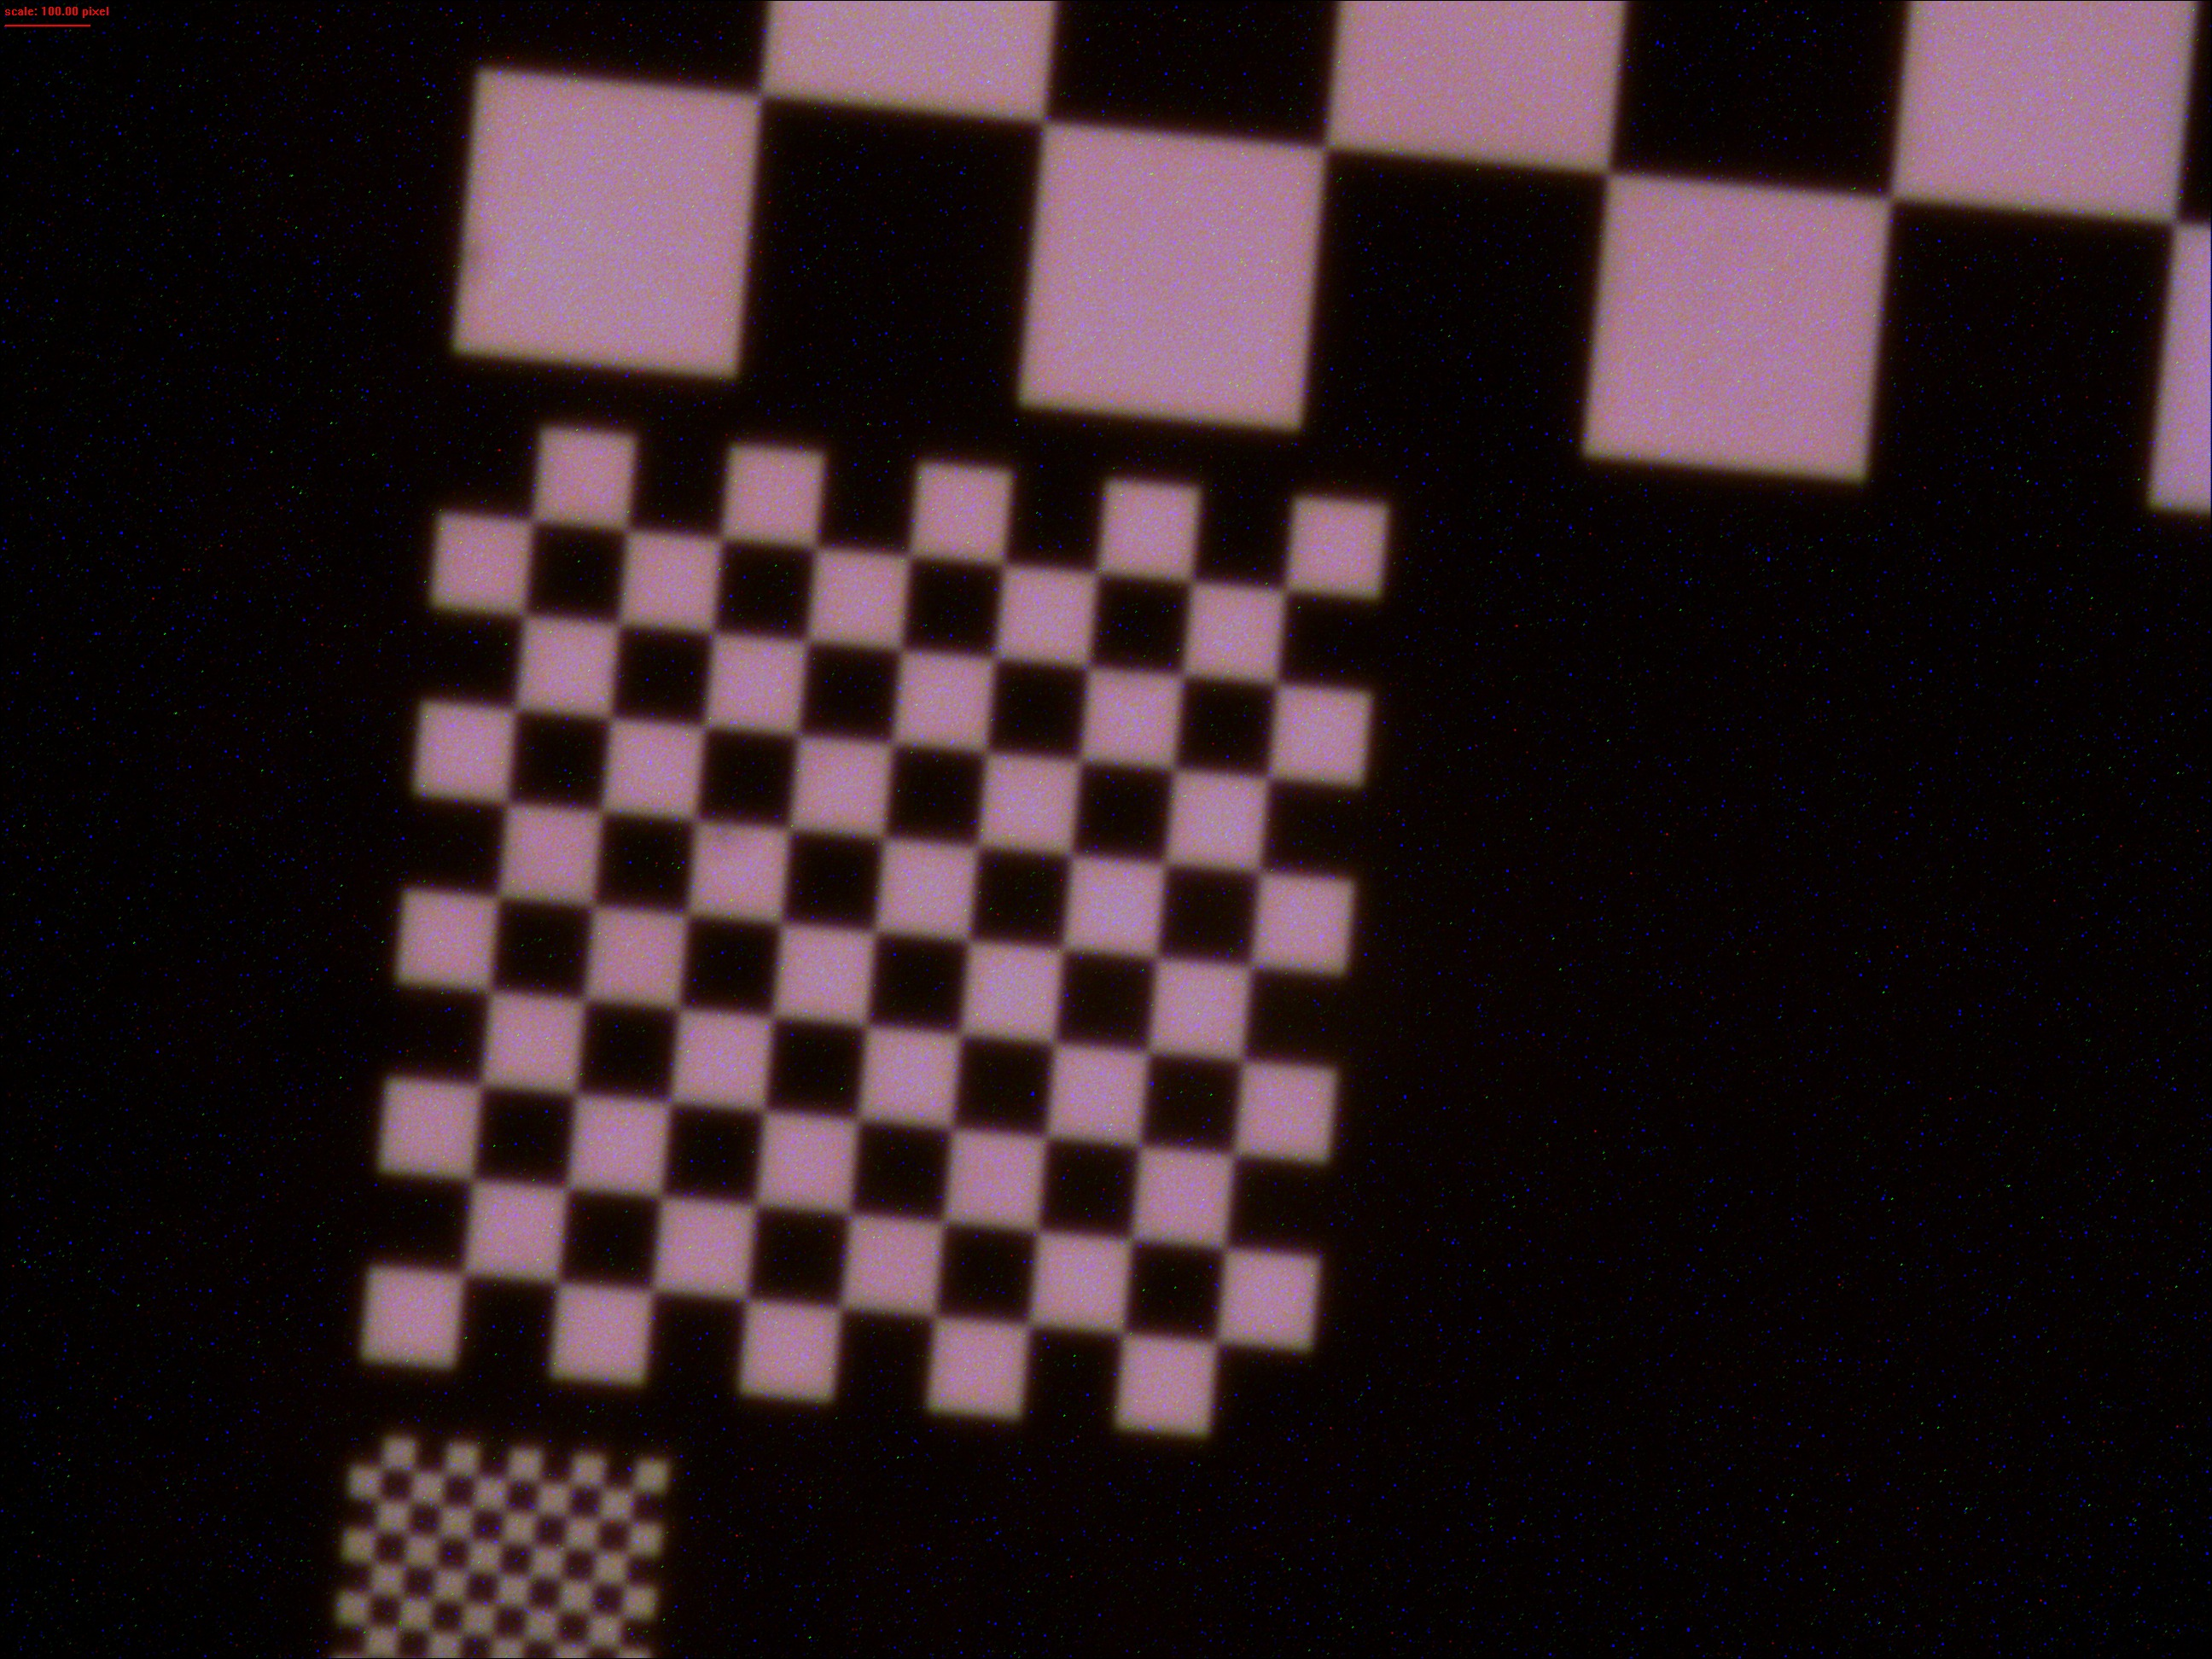
\includegraphics{data/mask/TS_05_20_13_51_30.jpg}}
%  	\caption{Mask}
%  	\label{fig:TS_05_20_13_51_30}
%  \end{subfigure}
%     \hfill
%     \begin{subfigure}[t]{0.24\linewidth}
%  	\centering
%  	\resizebox{\linewidth}{!}{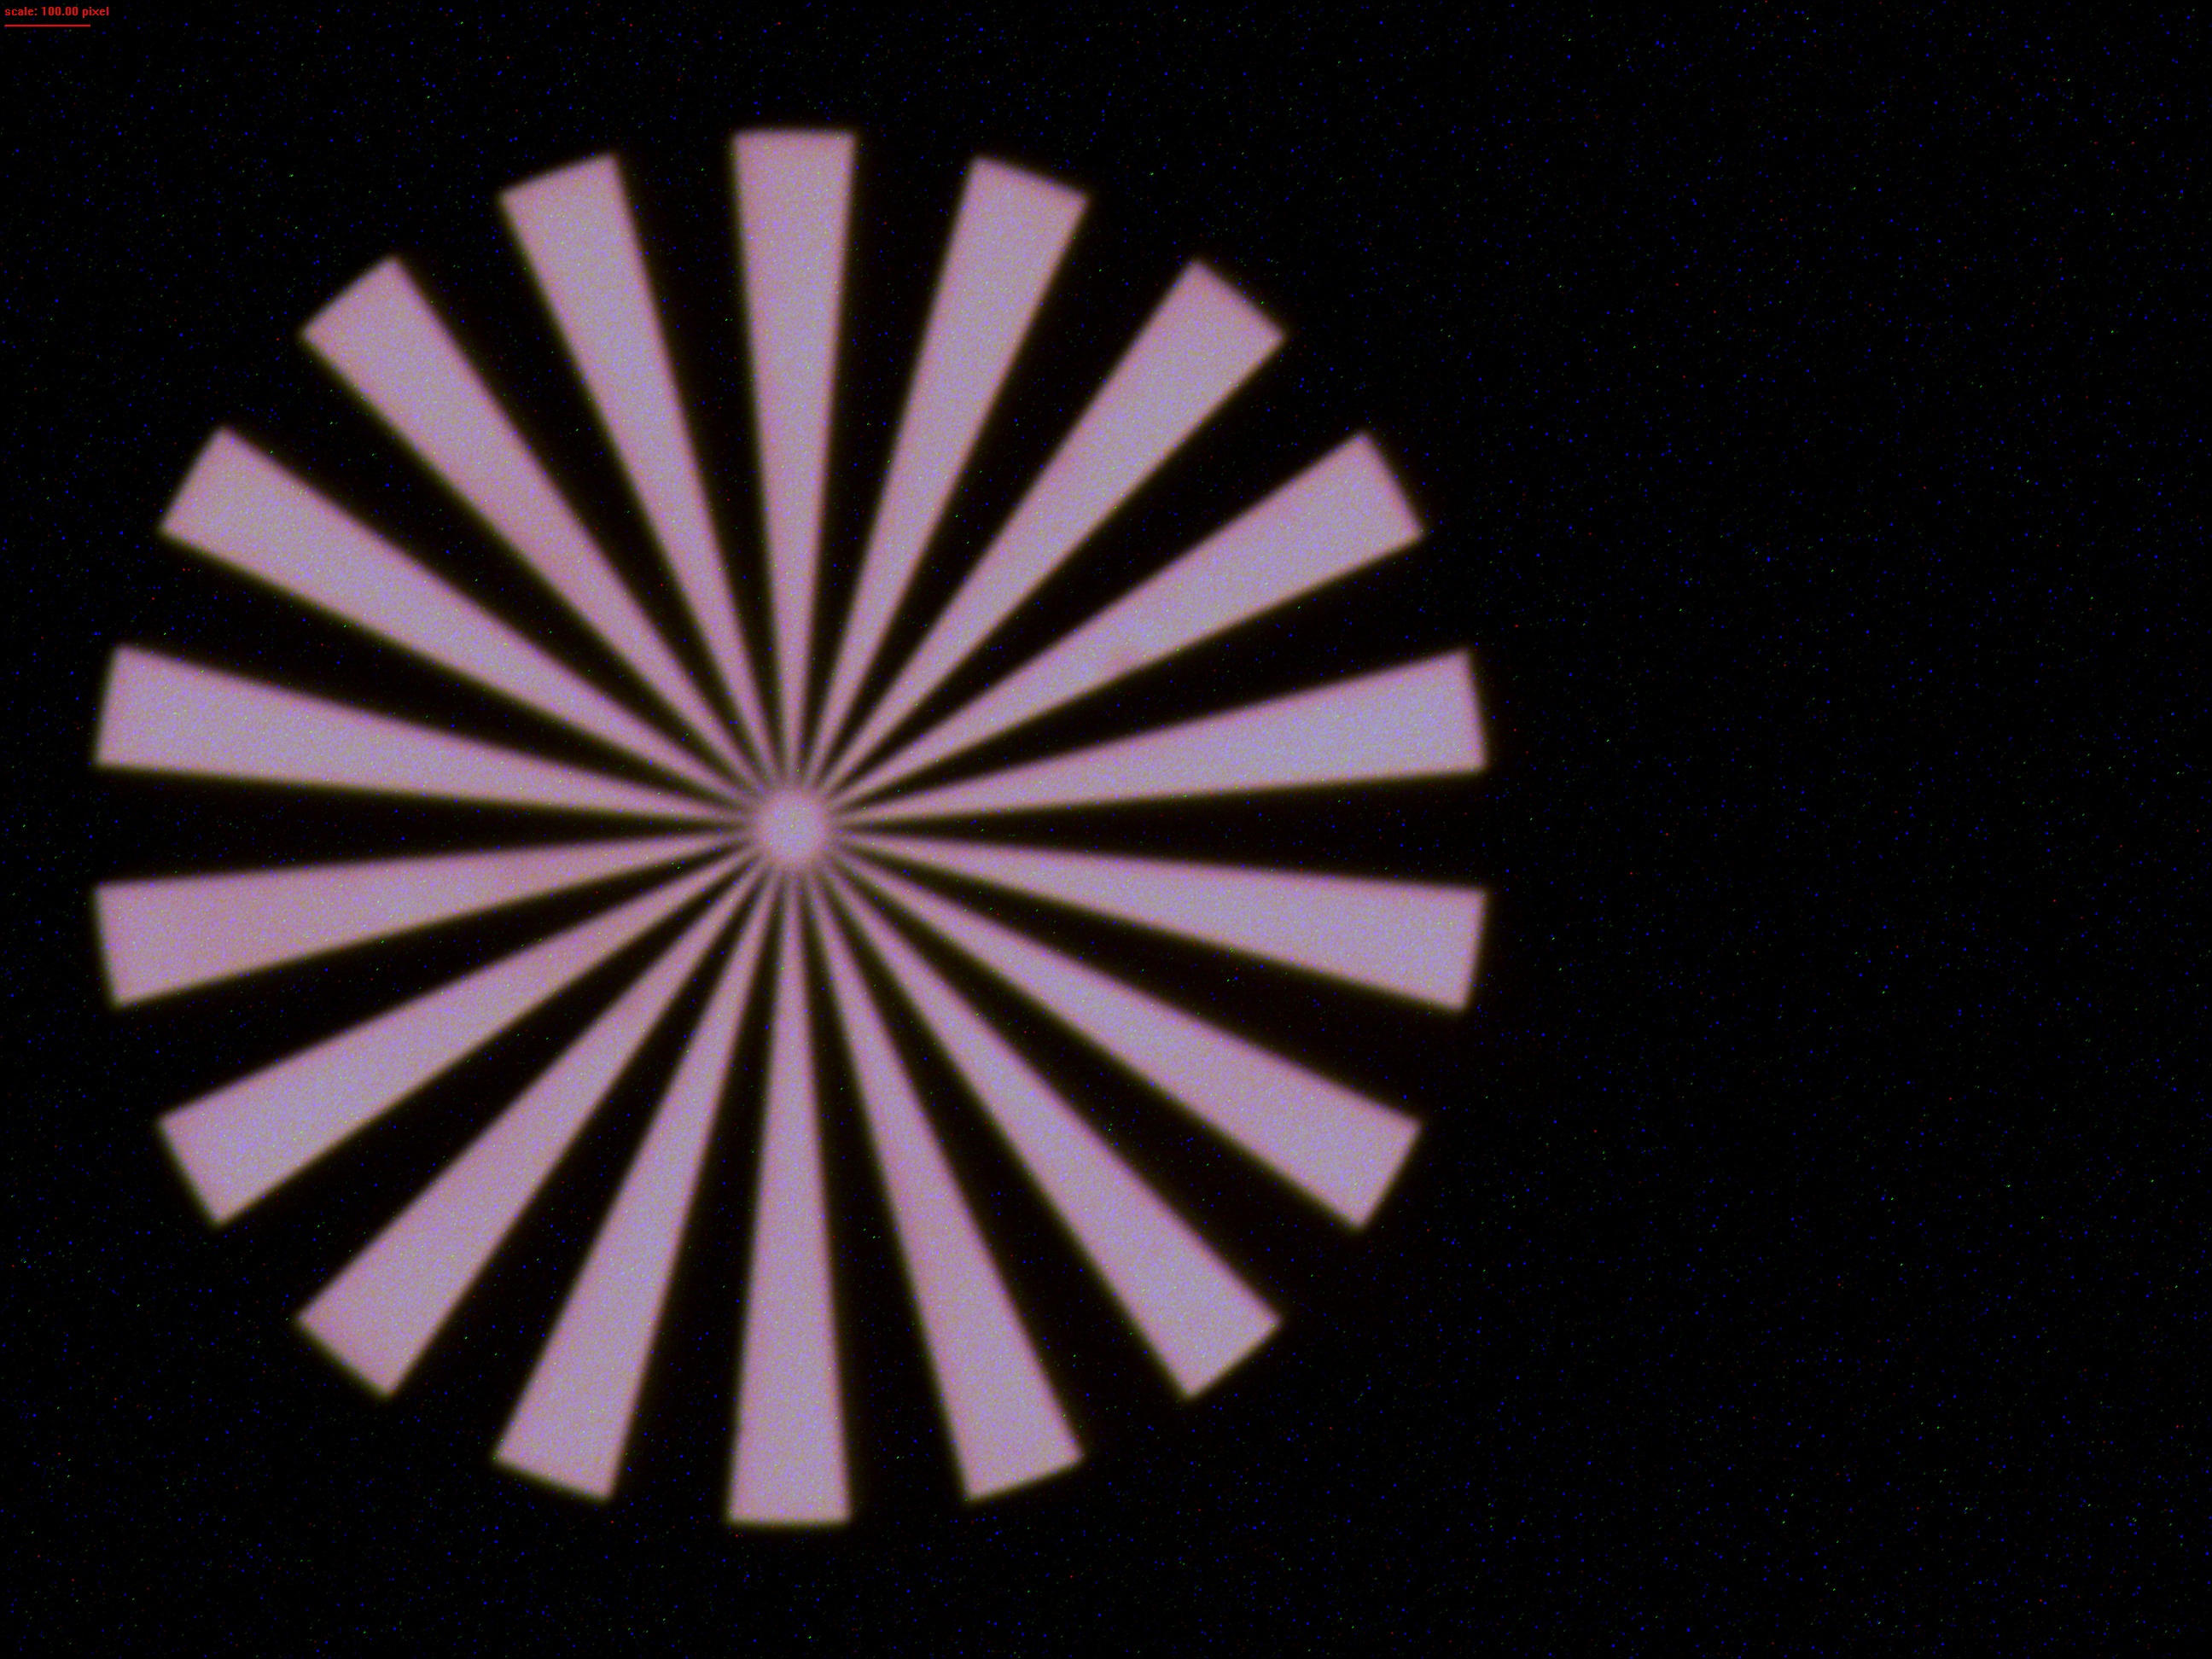
\includegraphics{data/mask/TS_05_20_13_52_44.jpg}}
%  	\caption{Mask}
%  	\label{fig:TS_05_20_13_52_44}
%  \end{subfigure}
% \end{figure*}


% \begin{figure*}[!t]	
%     \centering
%     \begin{subfigure}[t]{0.24\linewidth}
%  	\centering
%  	\resizebox{\linewidth}{!}{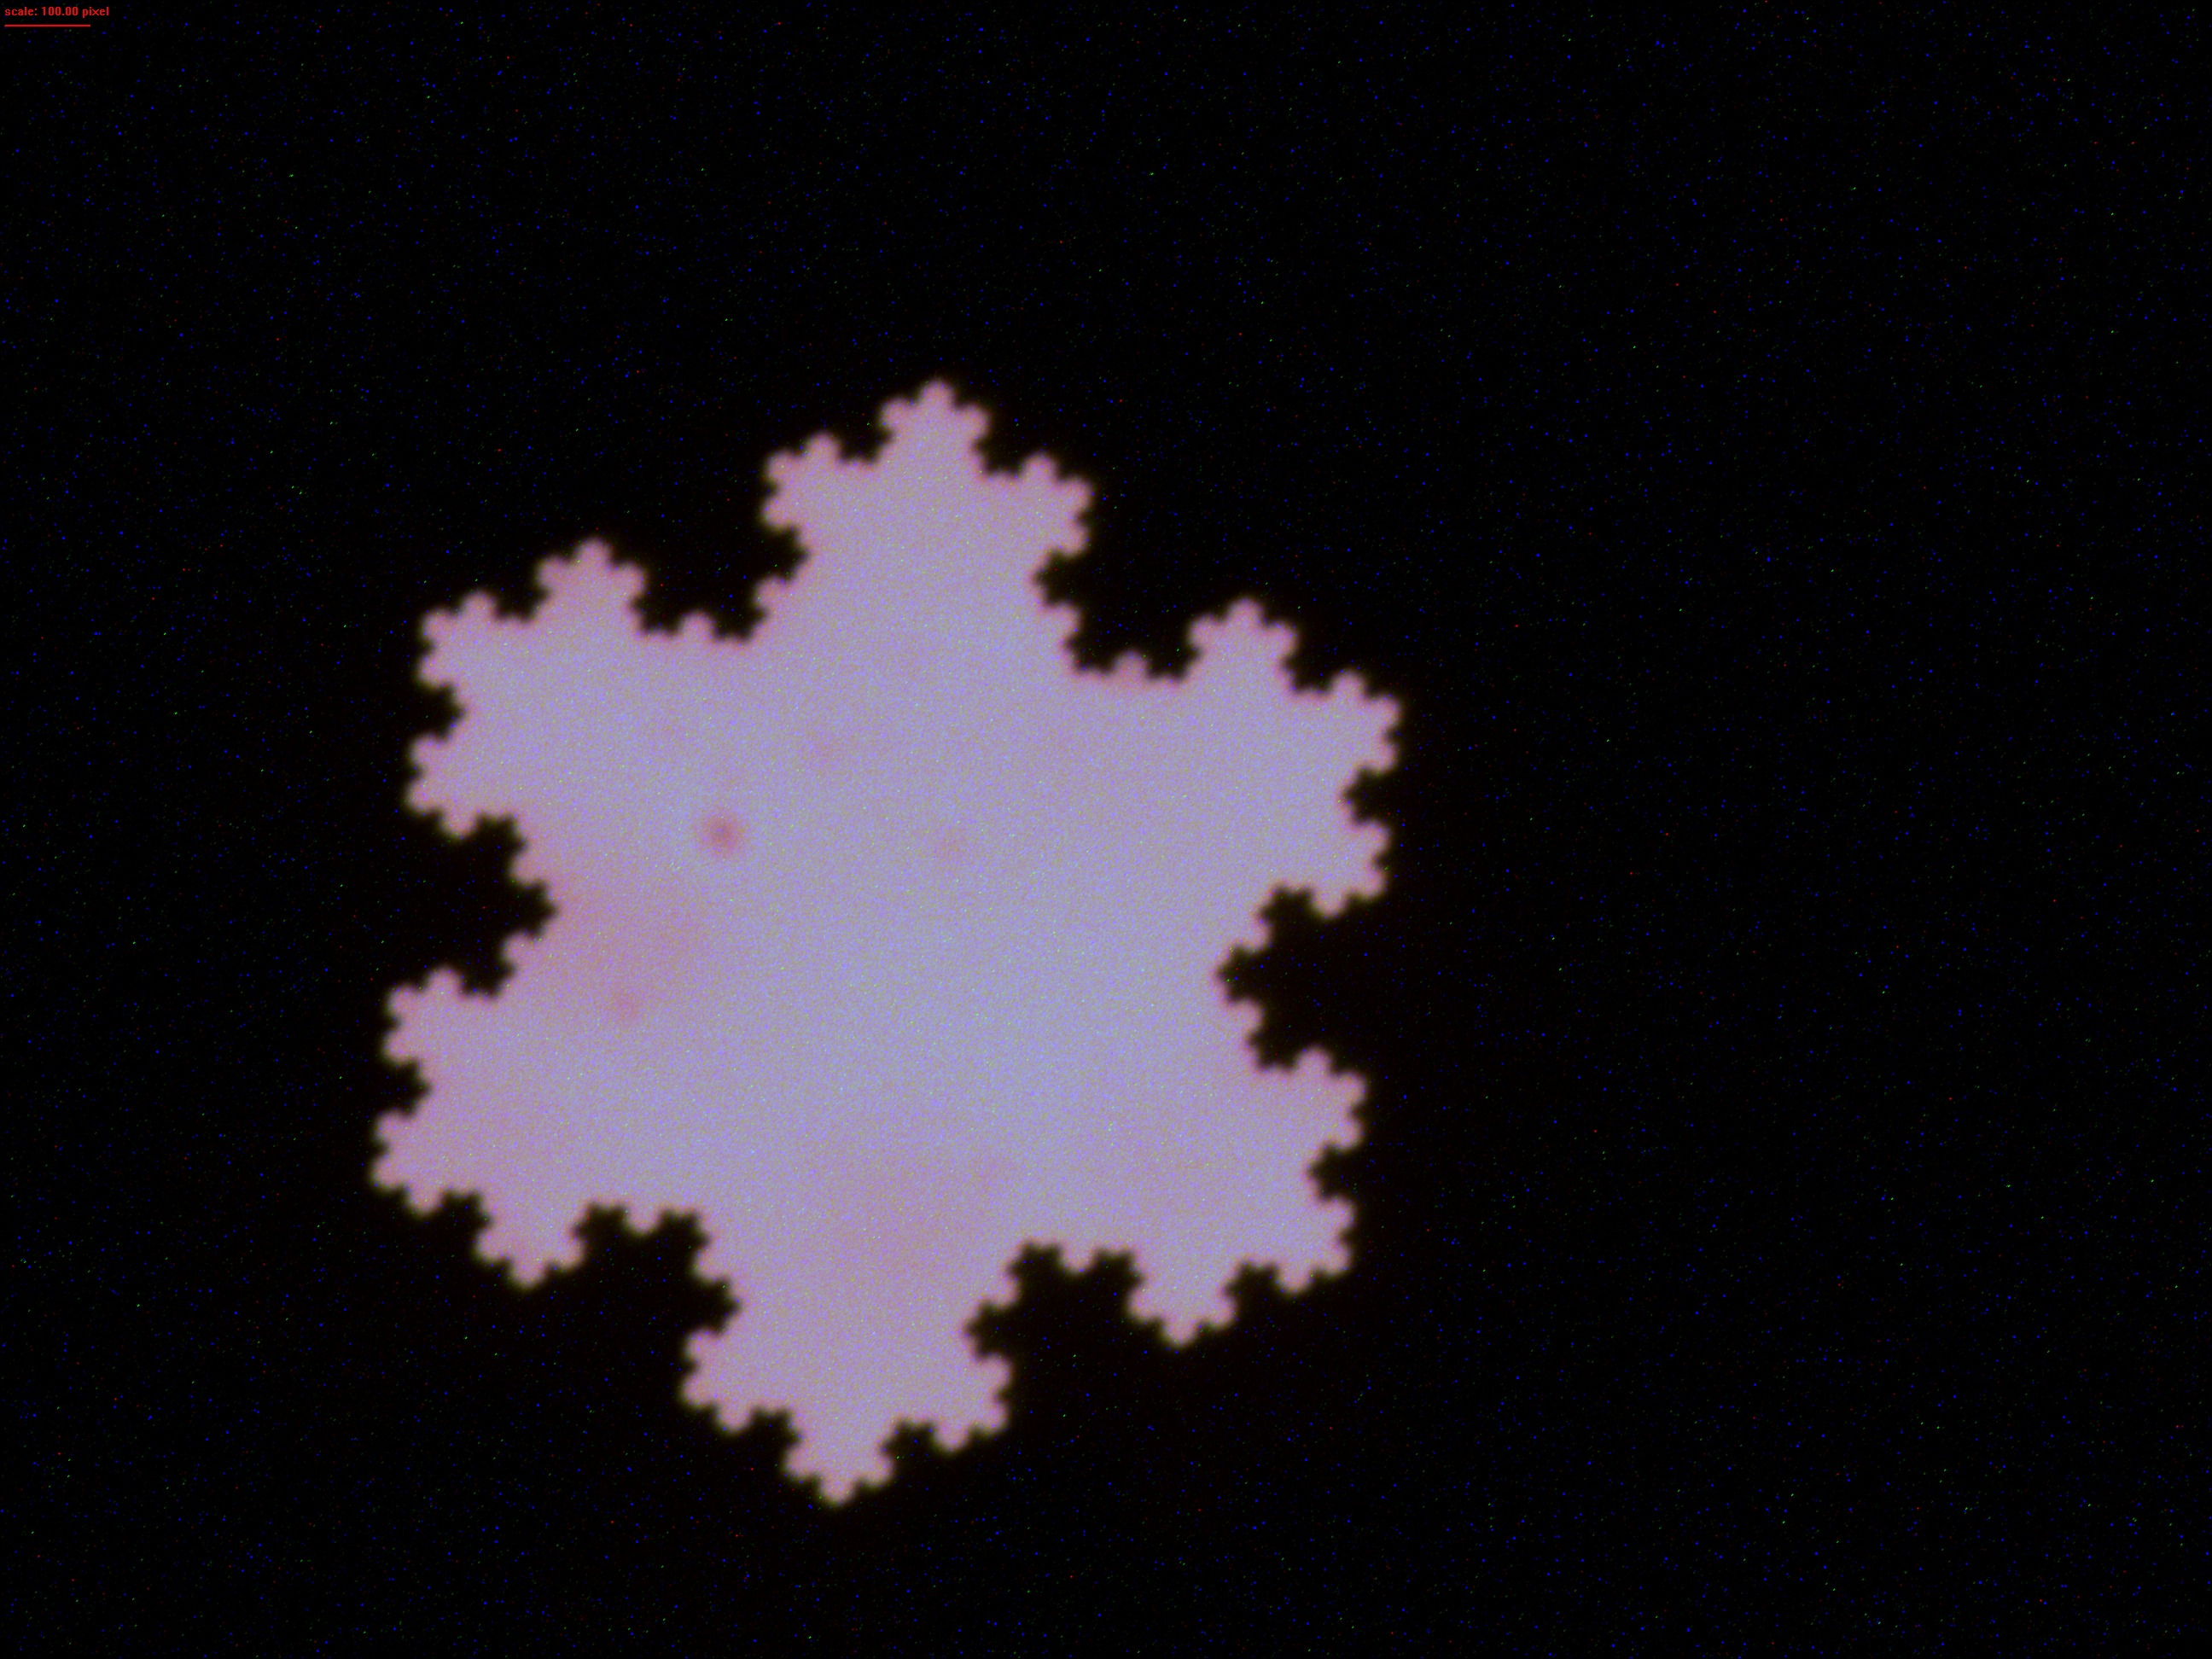
\includegraphics{data/mask/TS_05_20_13_53_38.jpg}}
%  	\caption{Mask}
%  	\label{fig:TS_05_20_13_53_38}
%  \end{subfigure}
%     \hfill
%     \begin{subfigure}[t]{0.24\linewidth}
%  	\centering
%  	\resizebox{\linewidth}{!}{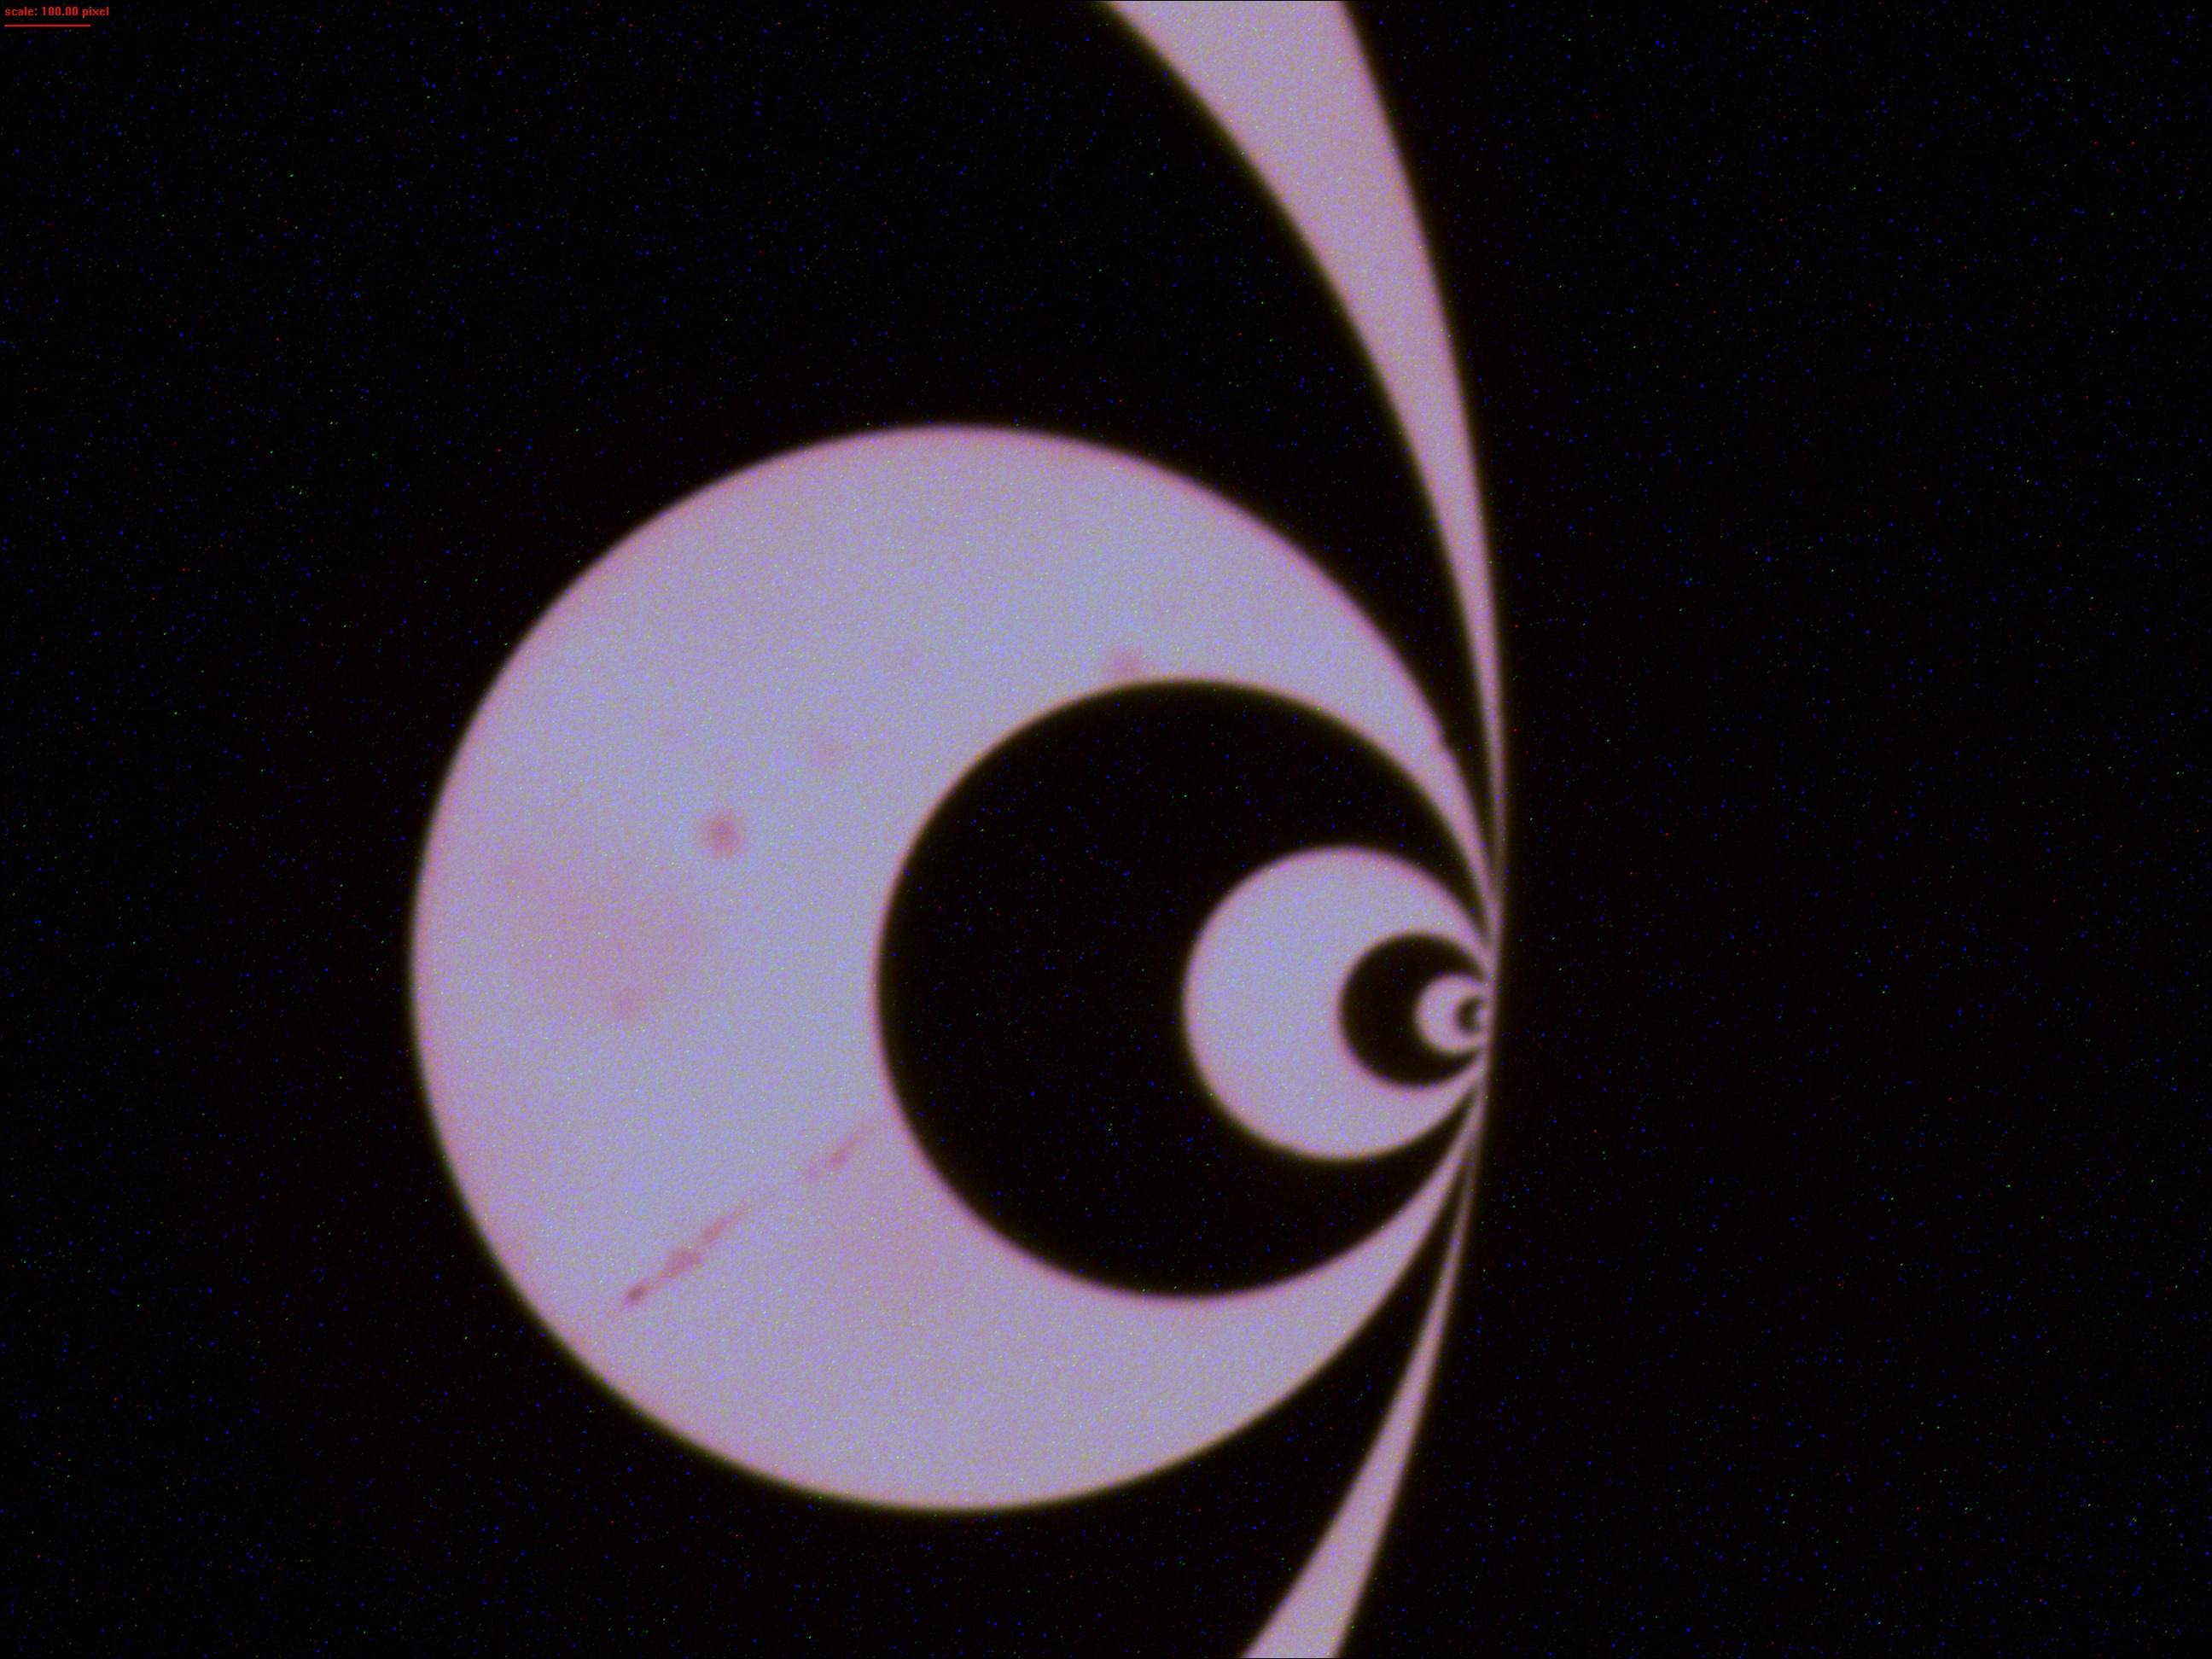
\includegraphics{data/mask/TS_05_20_13_54_28.jpg}}
%  	\caption{Mask}
%  	\label{fig:TS_05_20_13_54_28}
%  \end{subfigure}
%     \hfill
%     \begin{subfigure}[t]{0.24\linewidth}
%  	\centering
%  	\resizebox{\linewidth}{!}{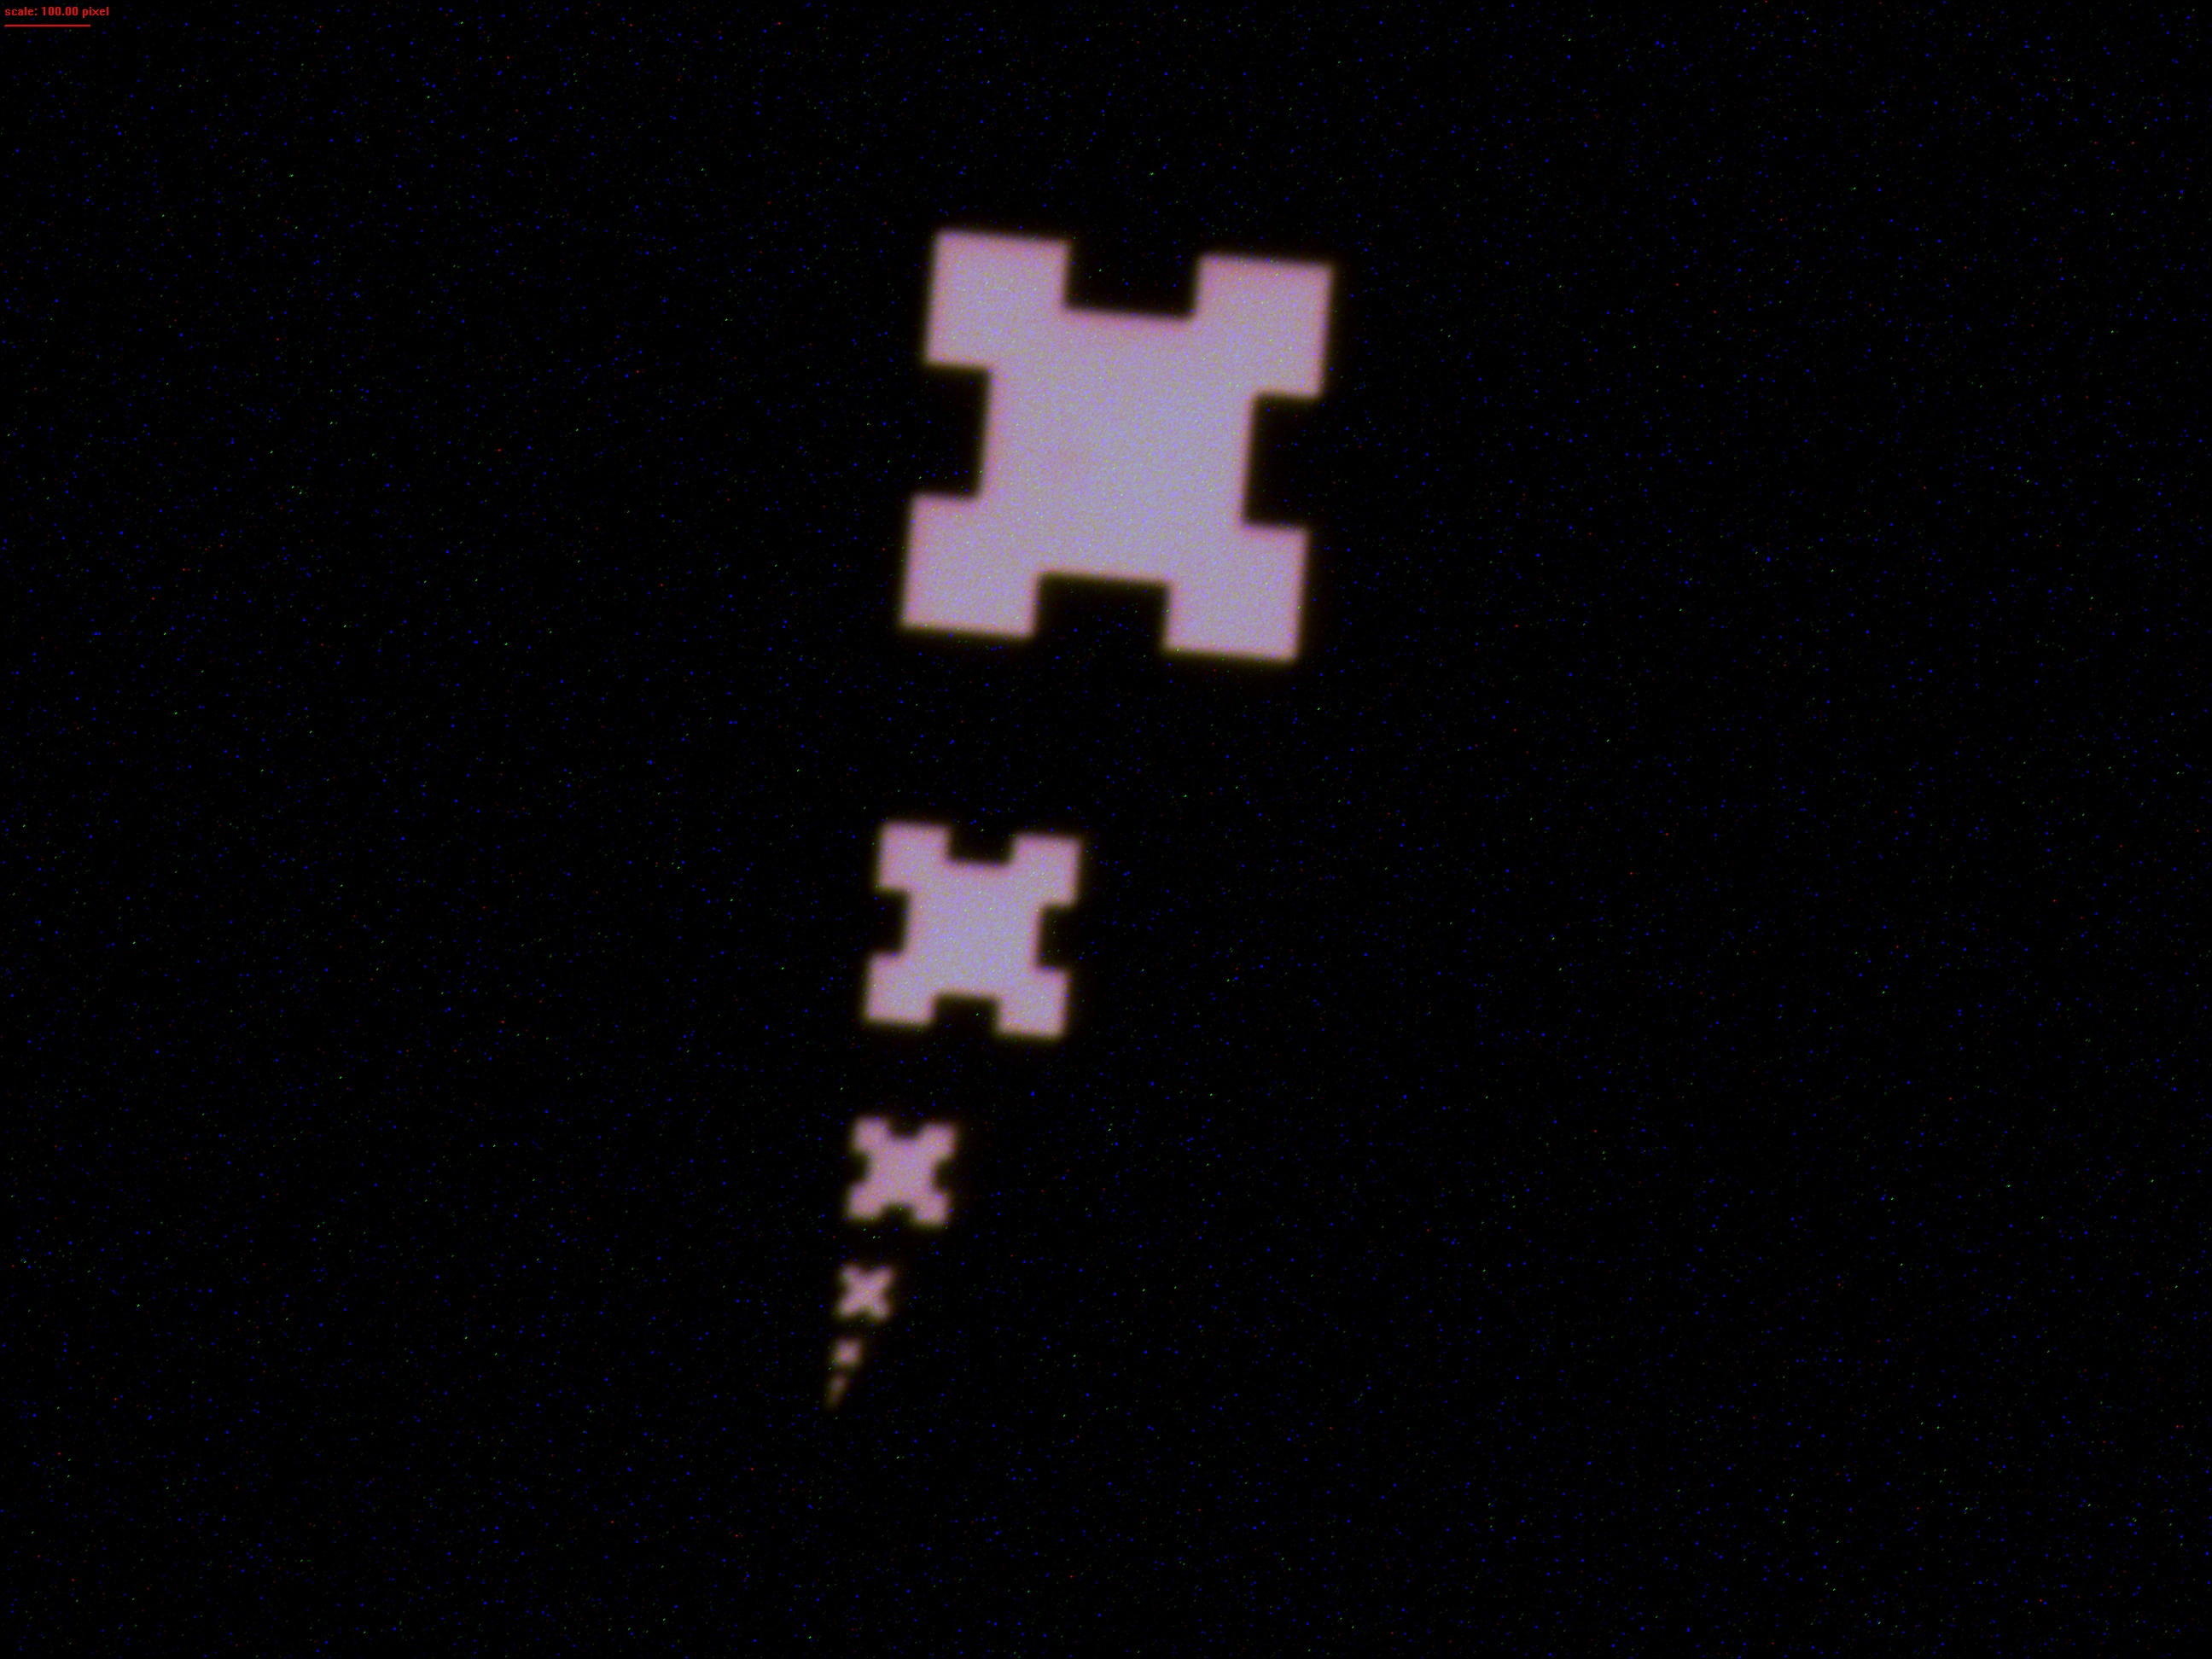
\includegraphics{data/mask/TS_05_20_13_54_51.jpg}}
%  	\caption{Mask}
%  	\label{fig:TS_05_20_13_54_51}
%  \end{subfigure}
% \hfill
%     \begin{subfigure}[t]{0.24\linewidth}
%  	\centering
%  	\resizebox{\linewidth}{!}{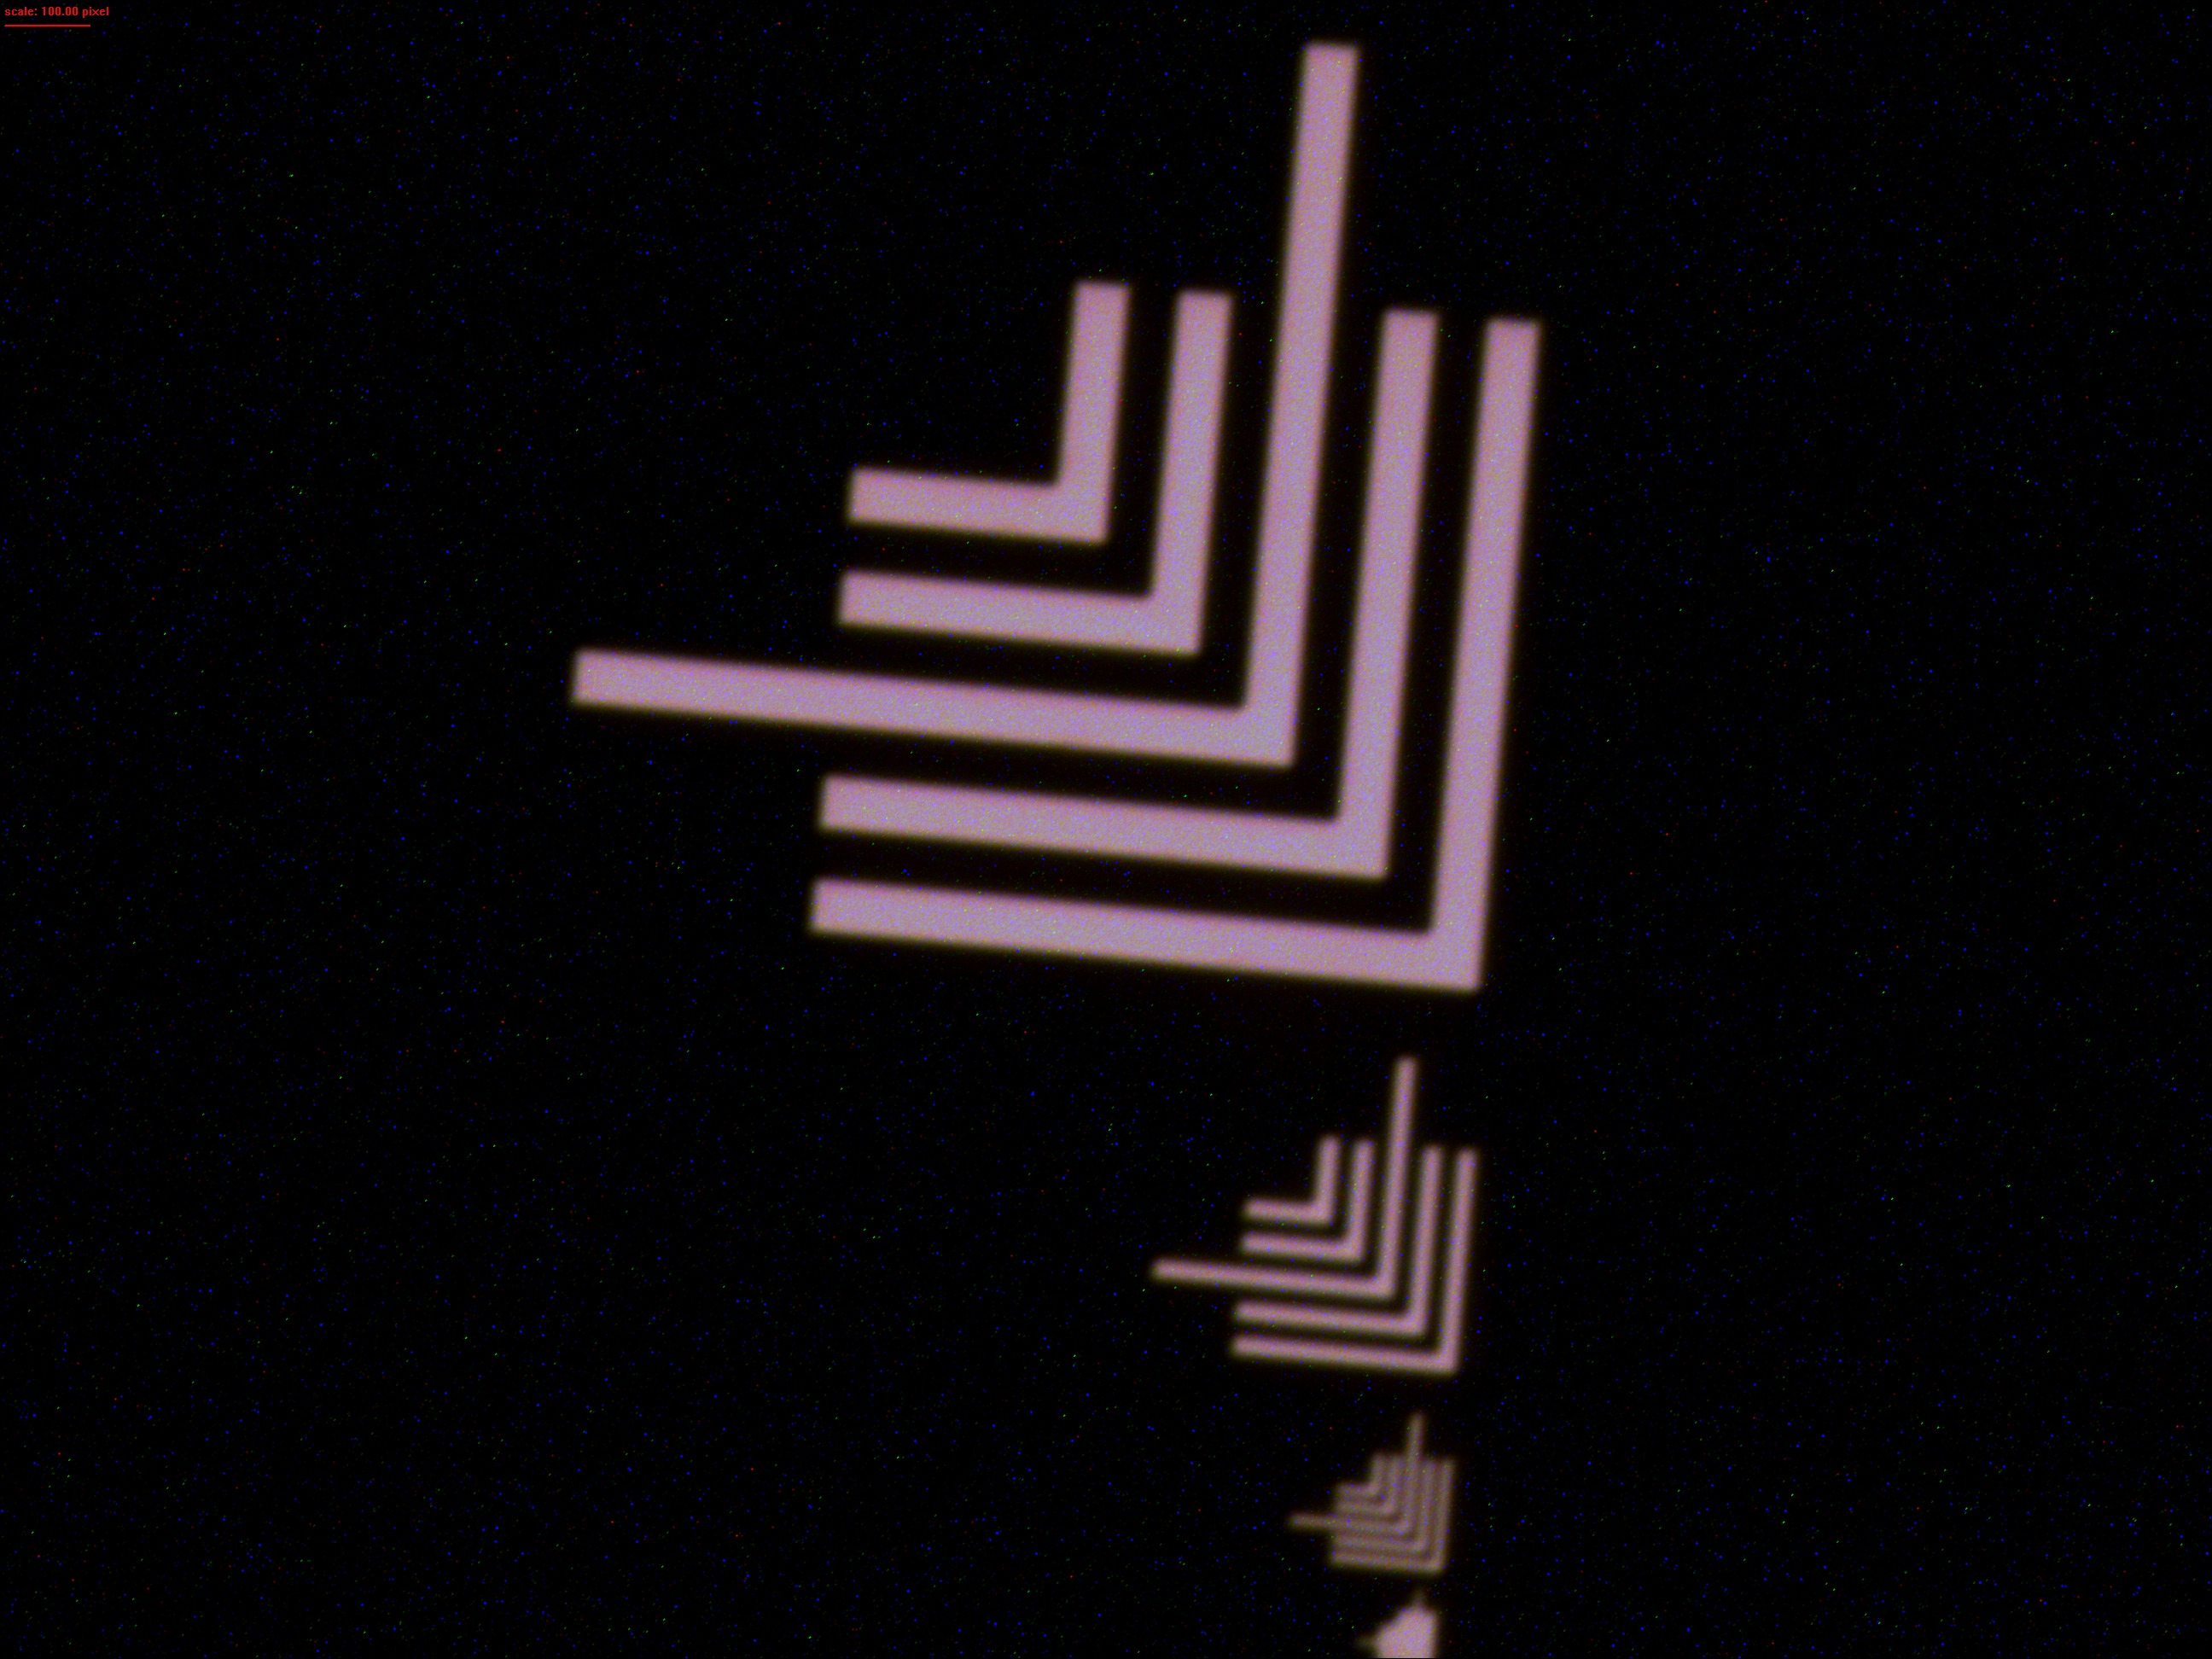
\includegraphics{data/mask/TS_05_20_13_55_57.jpg}}
%  	\caption{Mask}
%  	\label{fig:TS_05_20_13_55_57}
%  \end{subfigure}
% \end{figure*}

% % \todo[inline]{Optical microscope images of samples}
% \begin{figure*}[!t]	
%     \centering
%     \begin{subfigure}[t]{0.32\linewidth}
%  	\resizebox{\linewidth}{!}{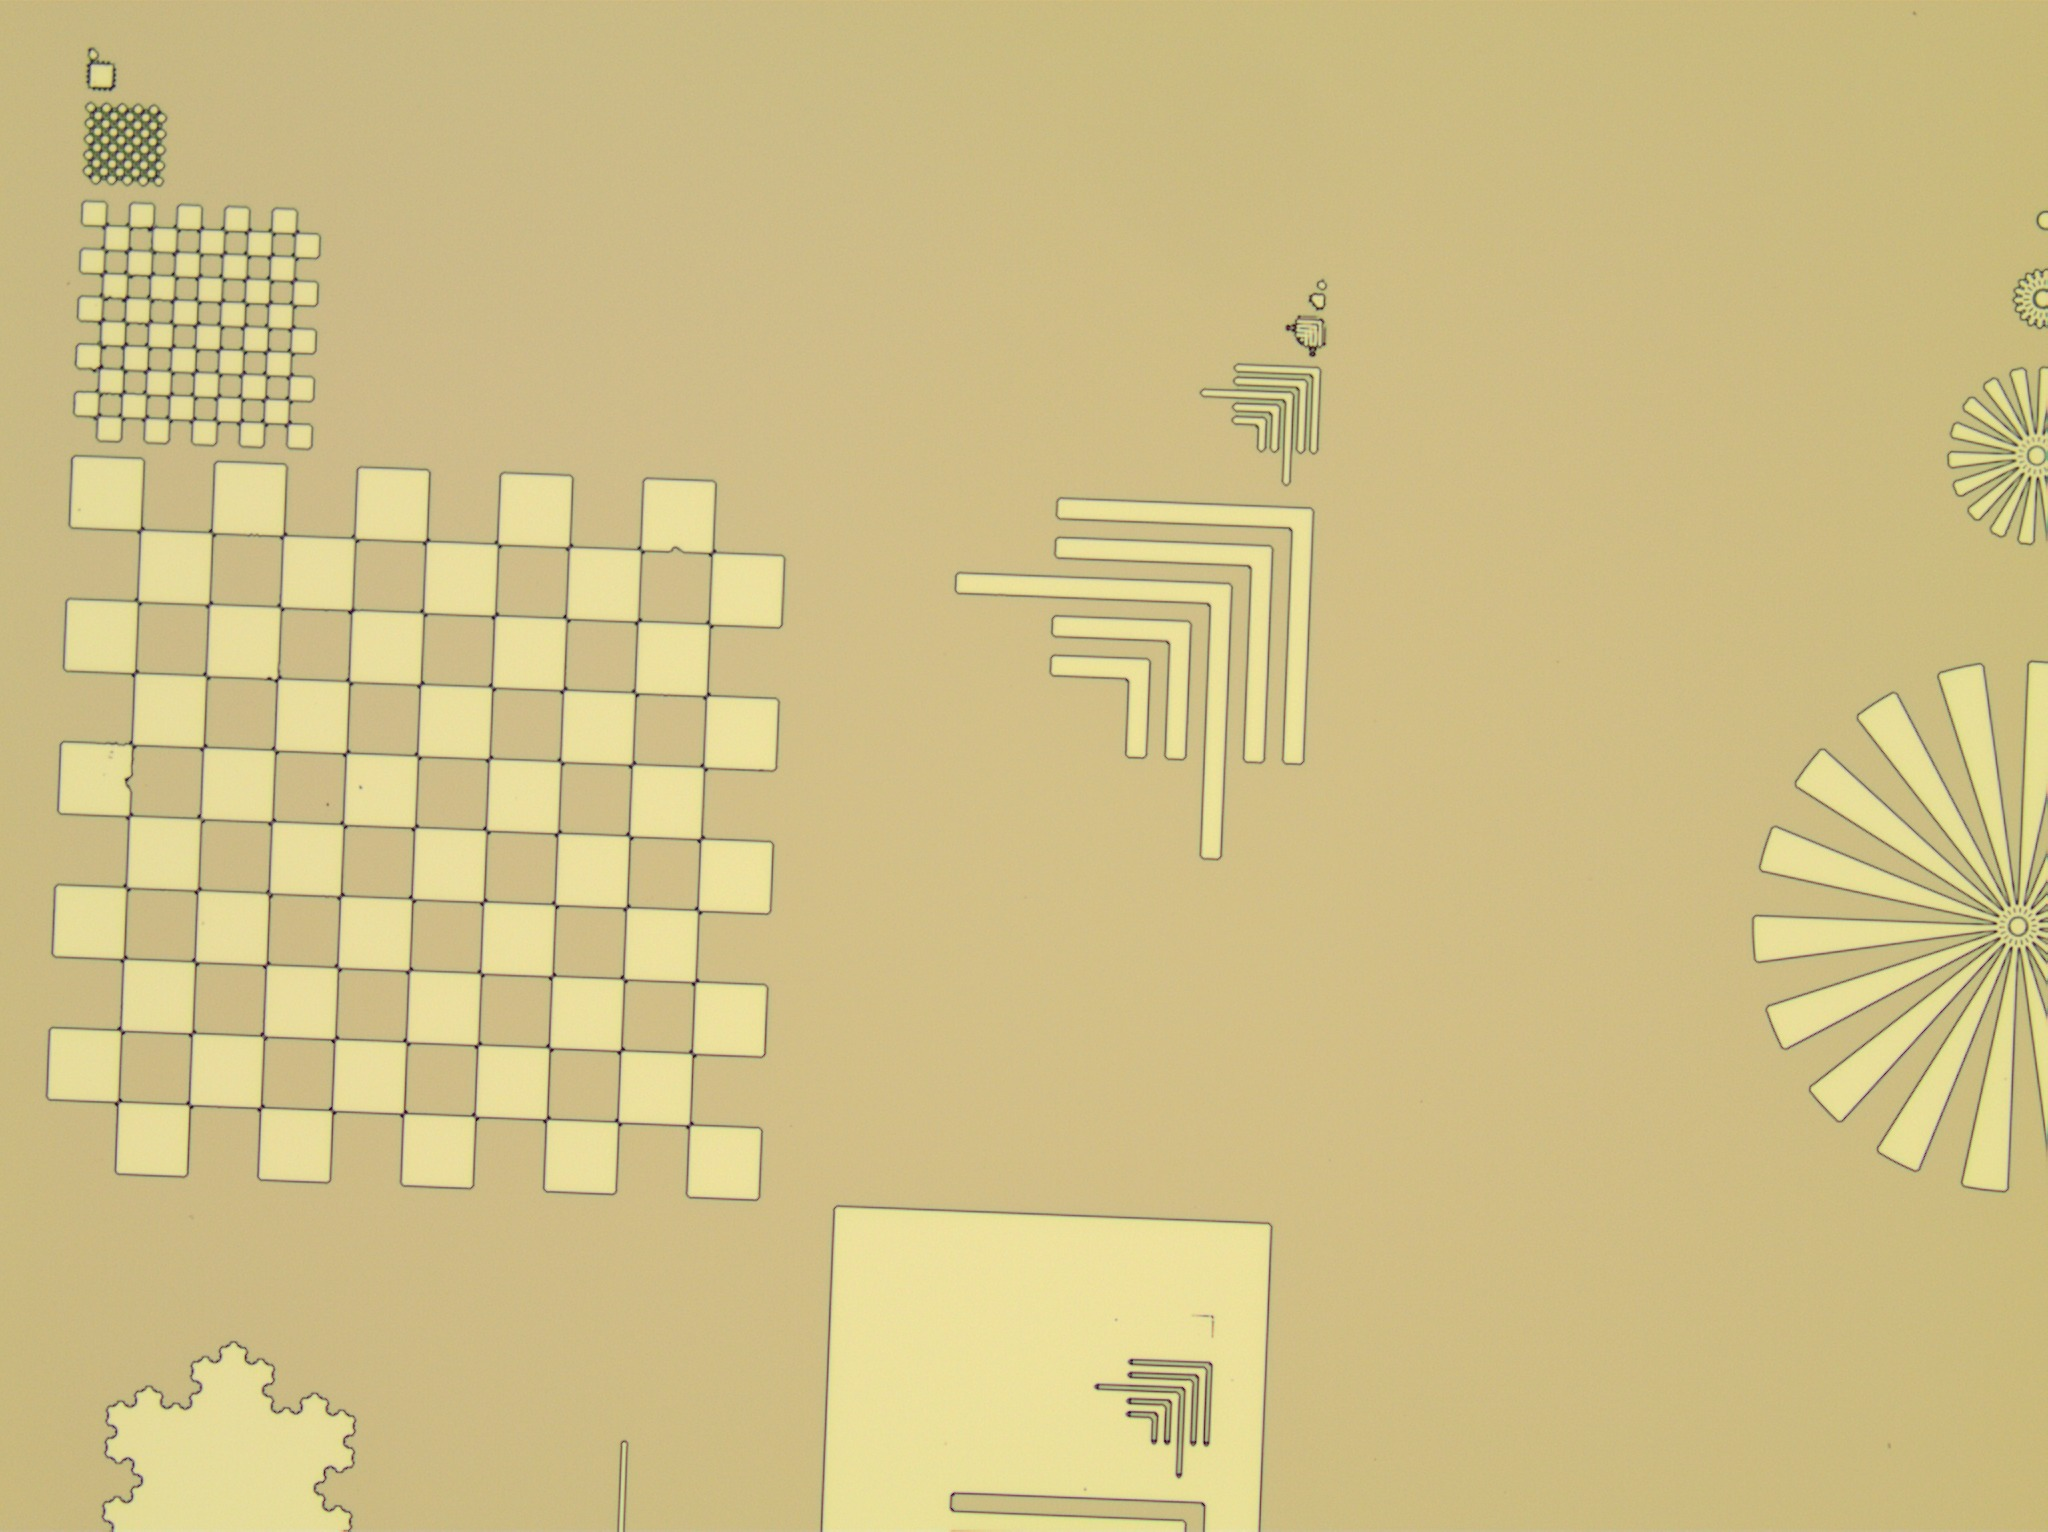
\includegraphics{data/b3b1.jpg}}
%  	\caption{b3b1}
%  	\label{fig:b3b1}
%  \end{subfigure}
% \hfill
%     \begin{subfigure}[t]{0.32\linewidth}
%  	\centering
%  	\resizebox{\linewidth}{!}{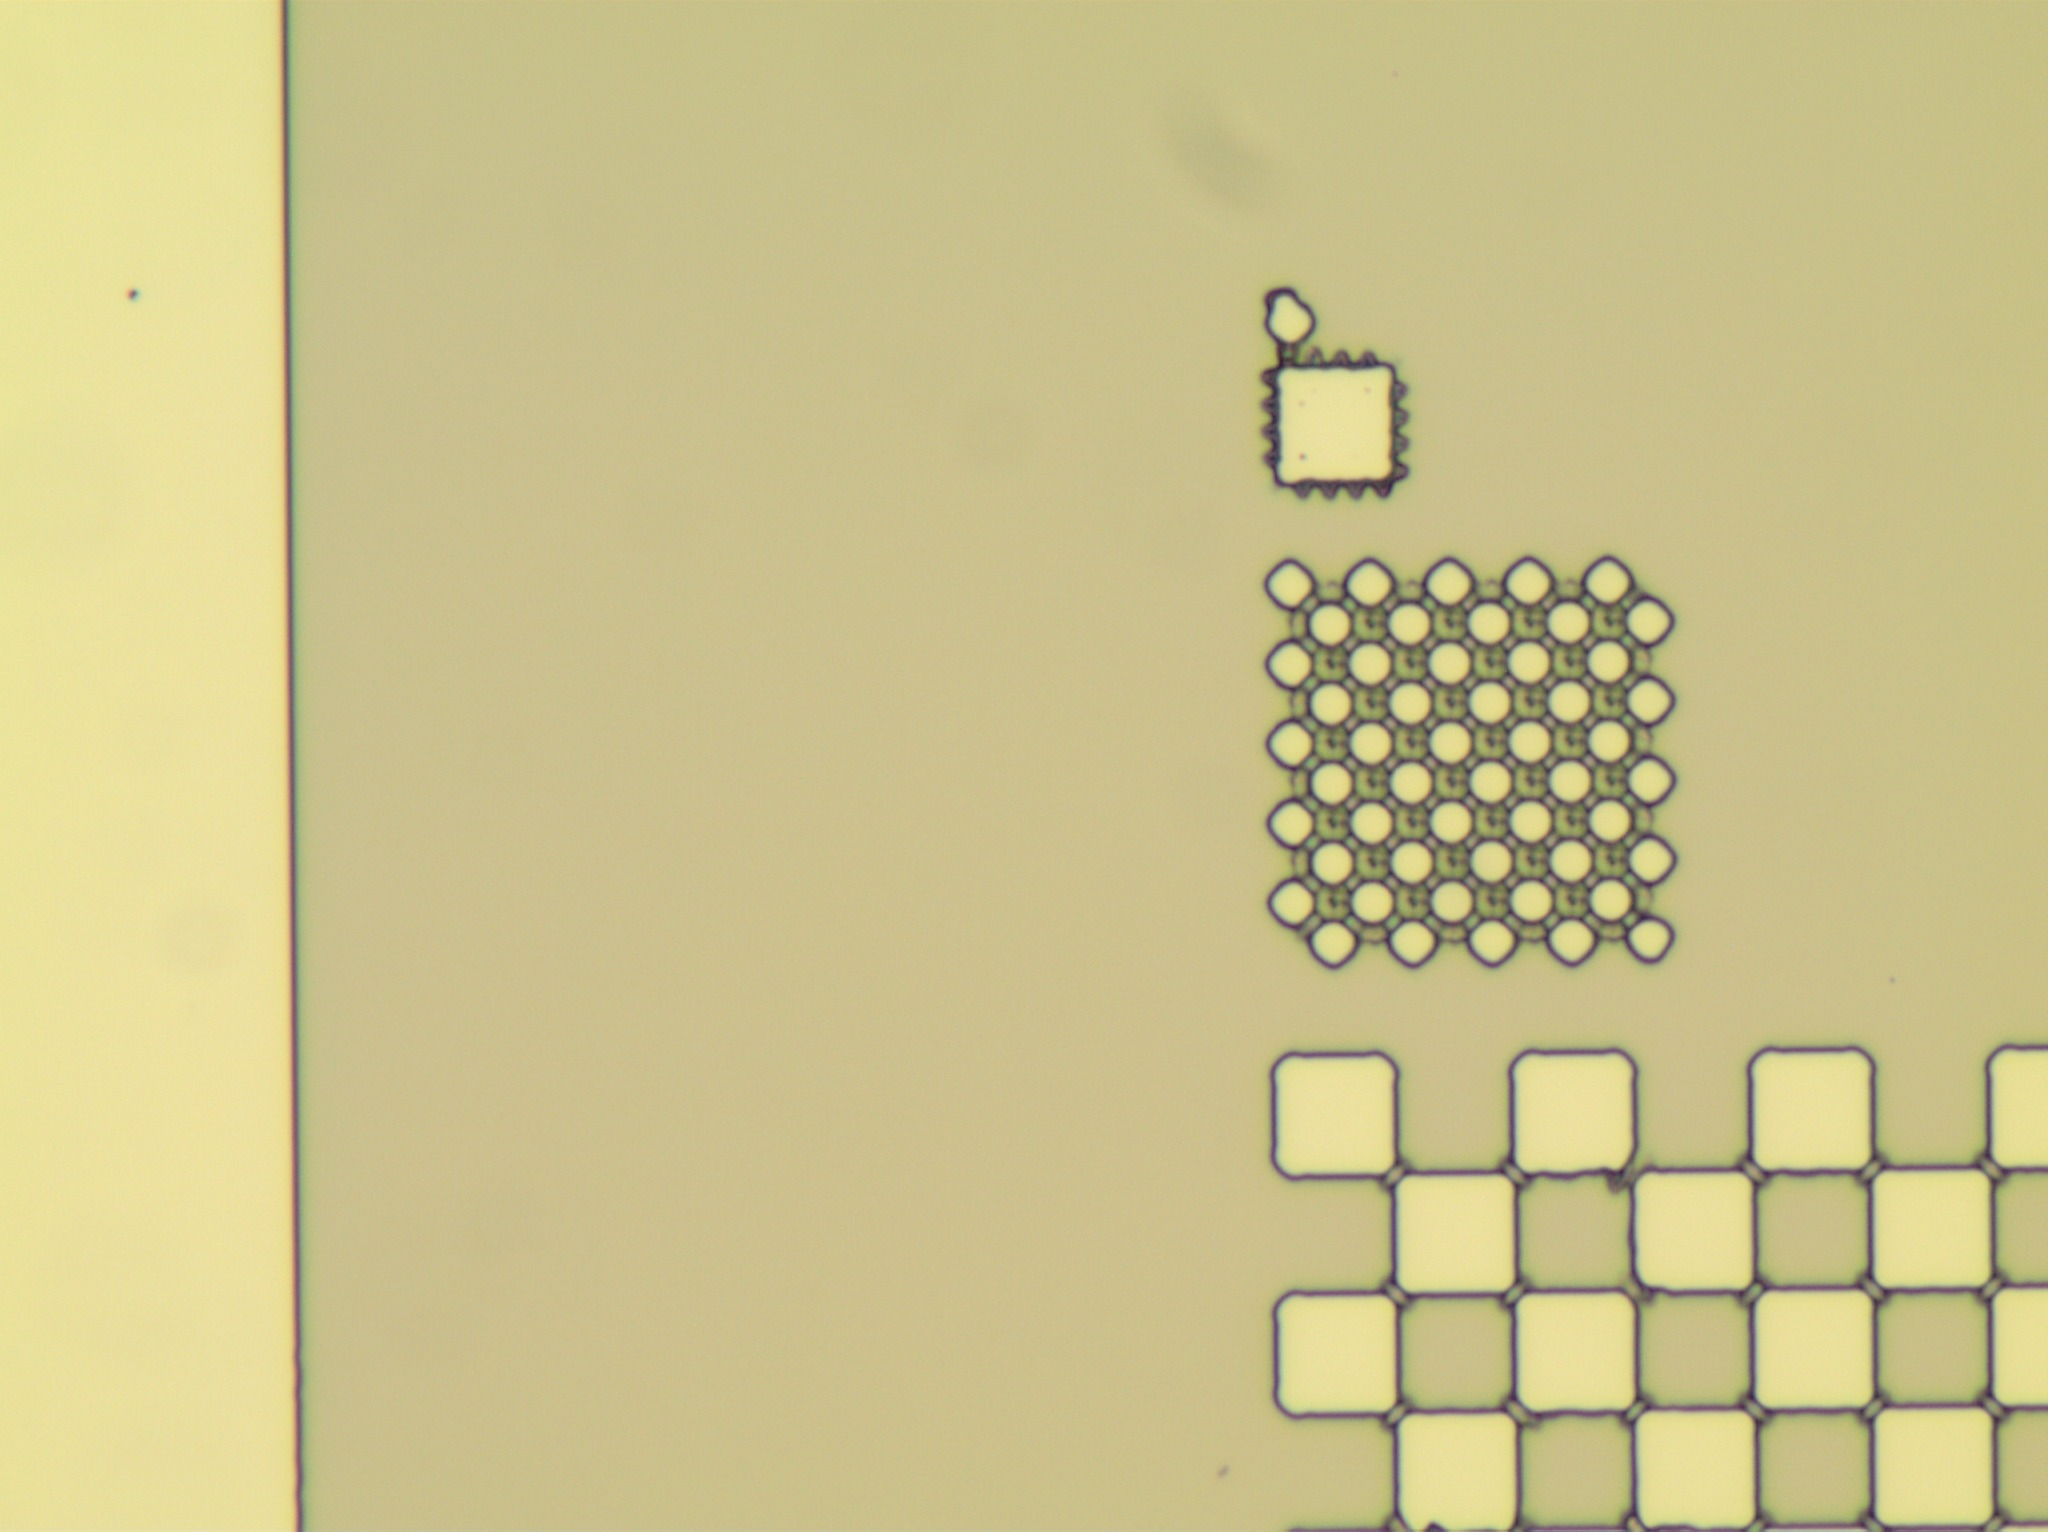
\includegraphics{data/b3b2.jpg}}
%  	\caption{b3b2}
%  	\label{fig:b3b2}
%  \end{subfigure}
% \hfill
%     \begin{subfigure}[t]{0.32\linewidth}
%  	\centering
%  	\resizebox{\linewidth}{!}{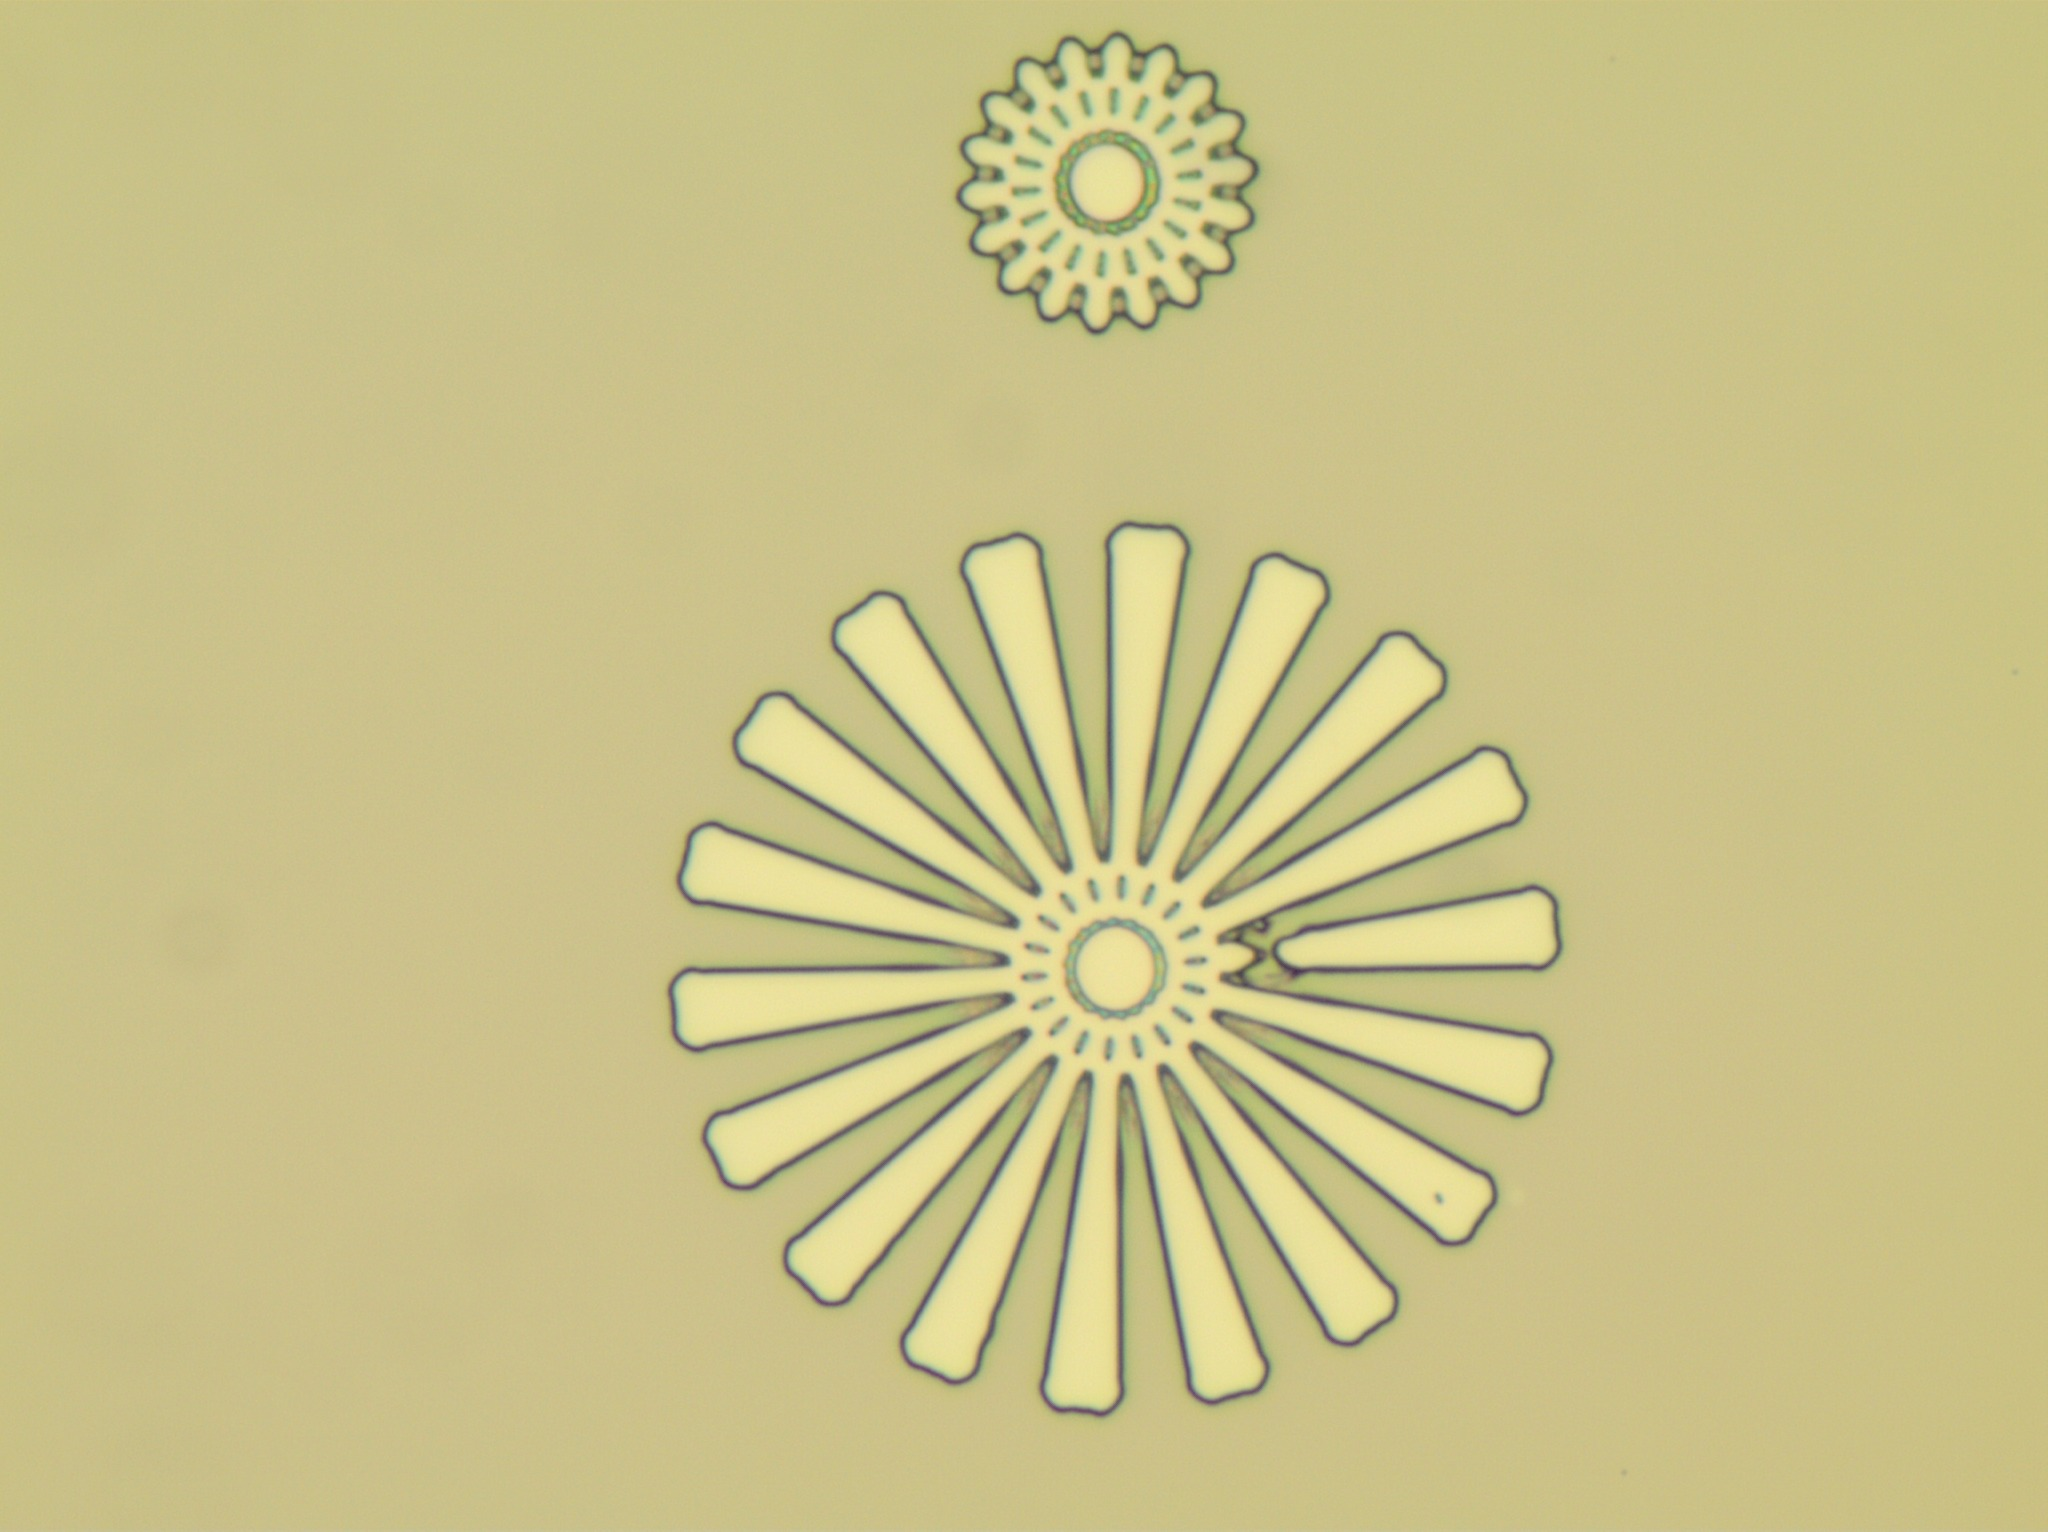
\includegraphics{data/b3b3.jpg}}
%  	\caption{b3b3}
%  	\label{fig:b3b3}
%  \end{subfigure}\\
%     \centering
%     \begin{subfigure}[t]{0.32\linewidth}
%  	\resizebox{\linewidth}{!}{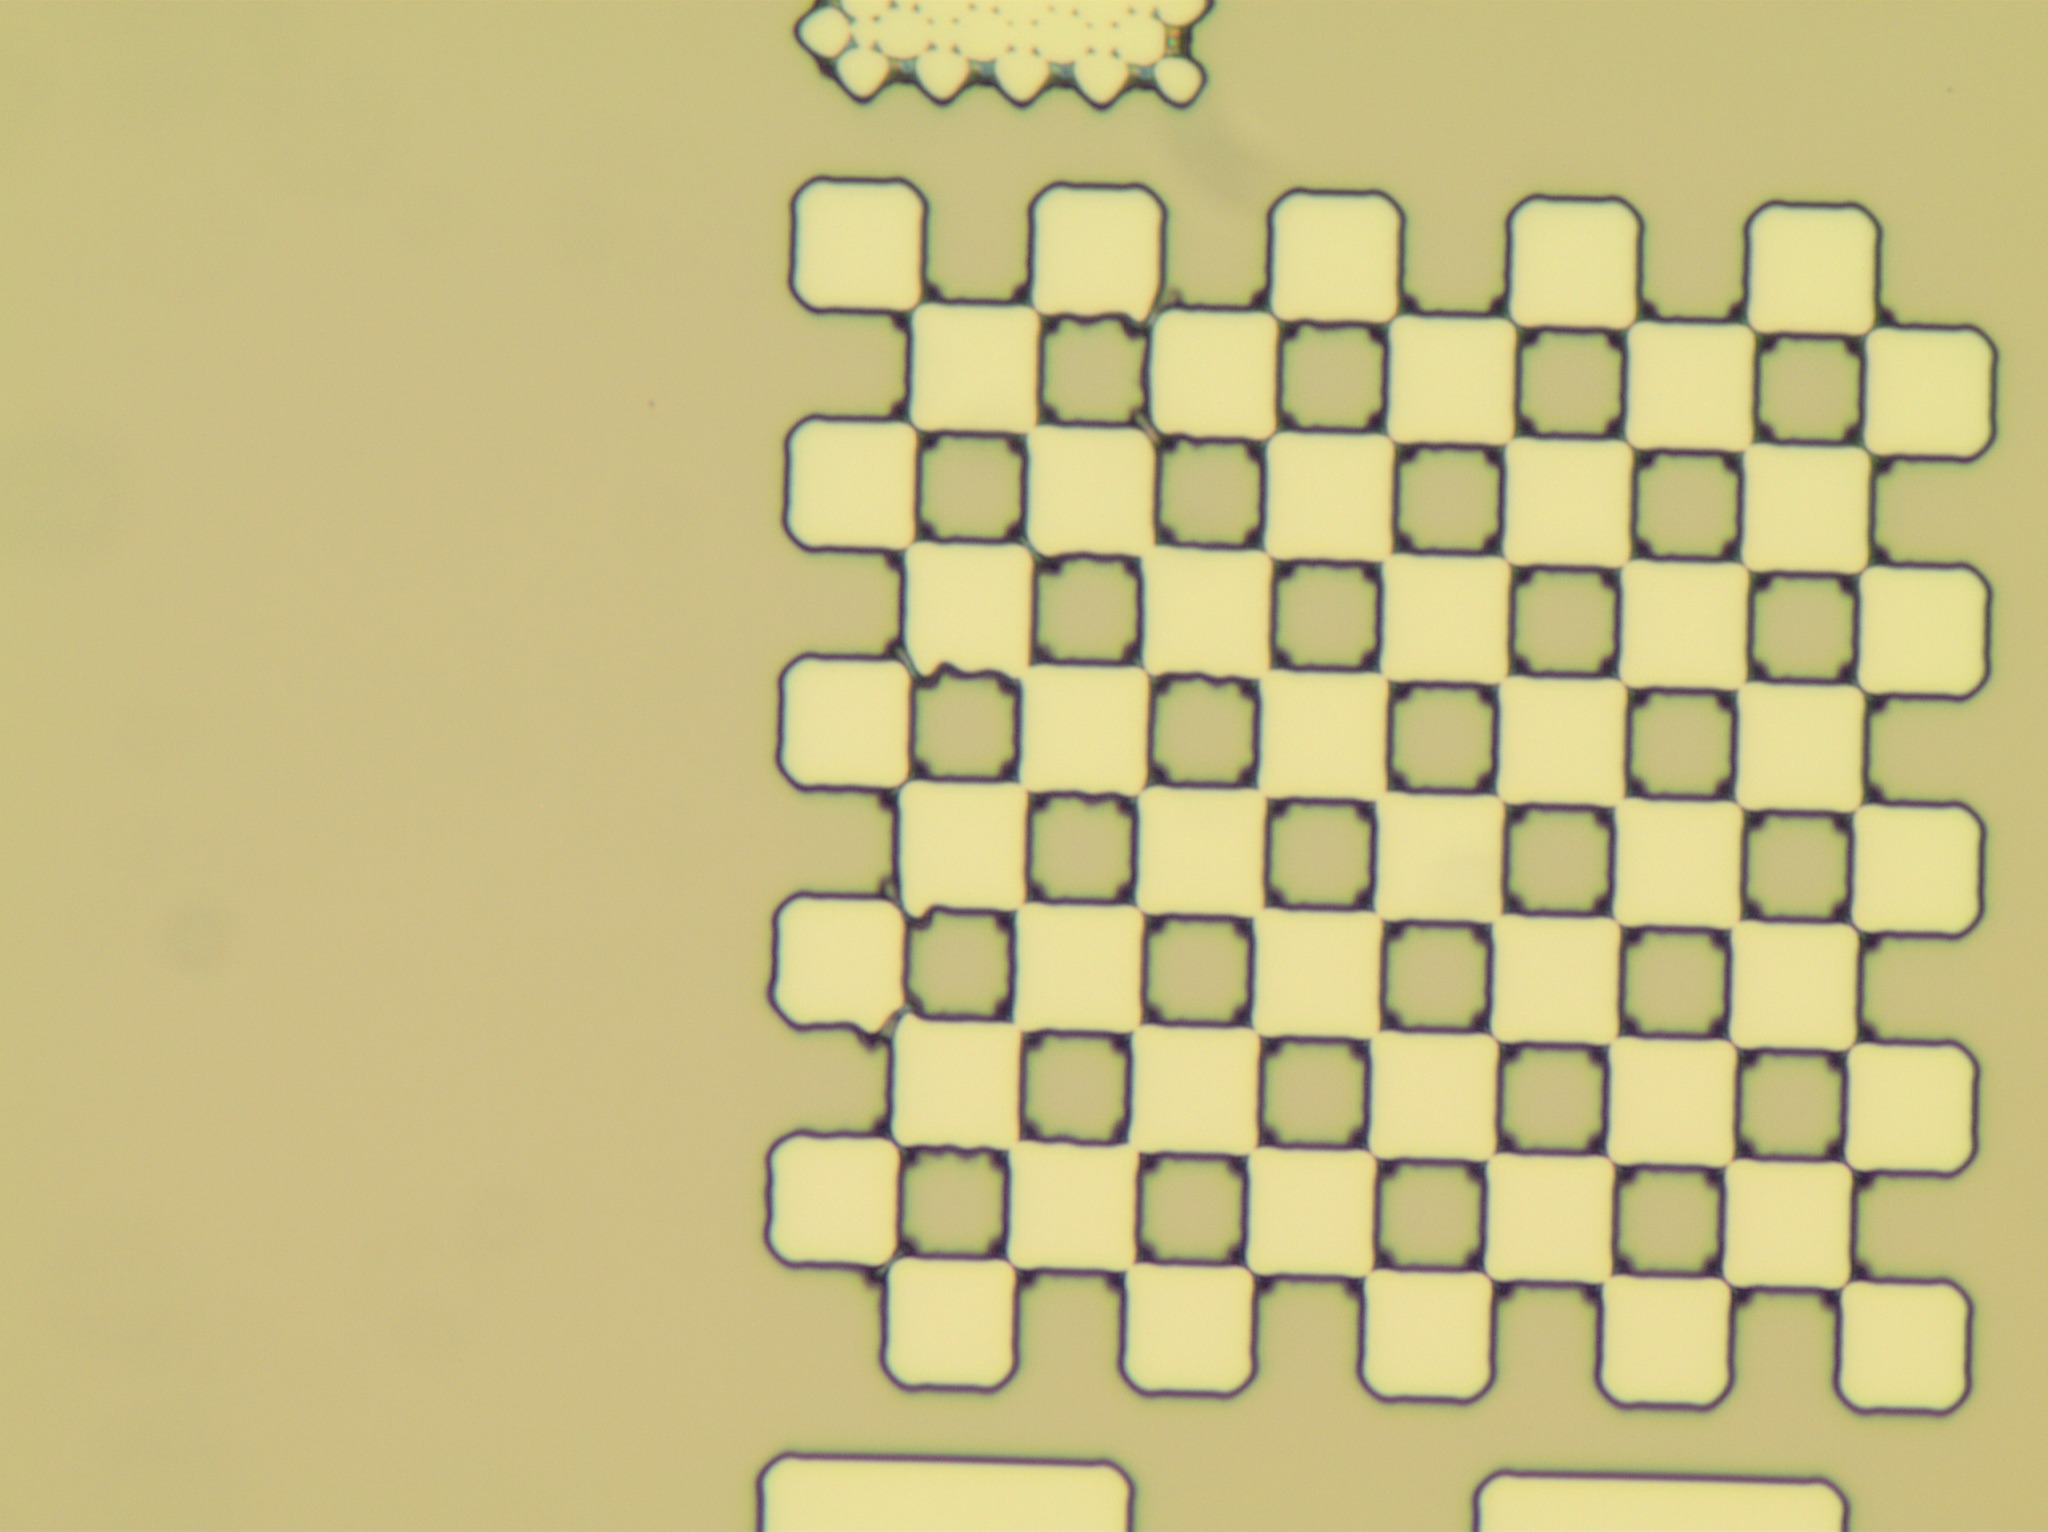
\includegraphics{data/b3c1.jpg}}
%  	\caption{b3c1}
%  	\label{fig:b3c1}
%  \end{subfigure}
% \hspace{10mm}
% \begin{subfigure}[t]{0.32\linewidth}
%  	\centering
%  	\resizebox{\linewidth}{!}{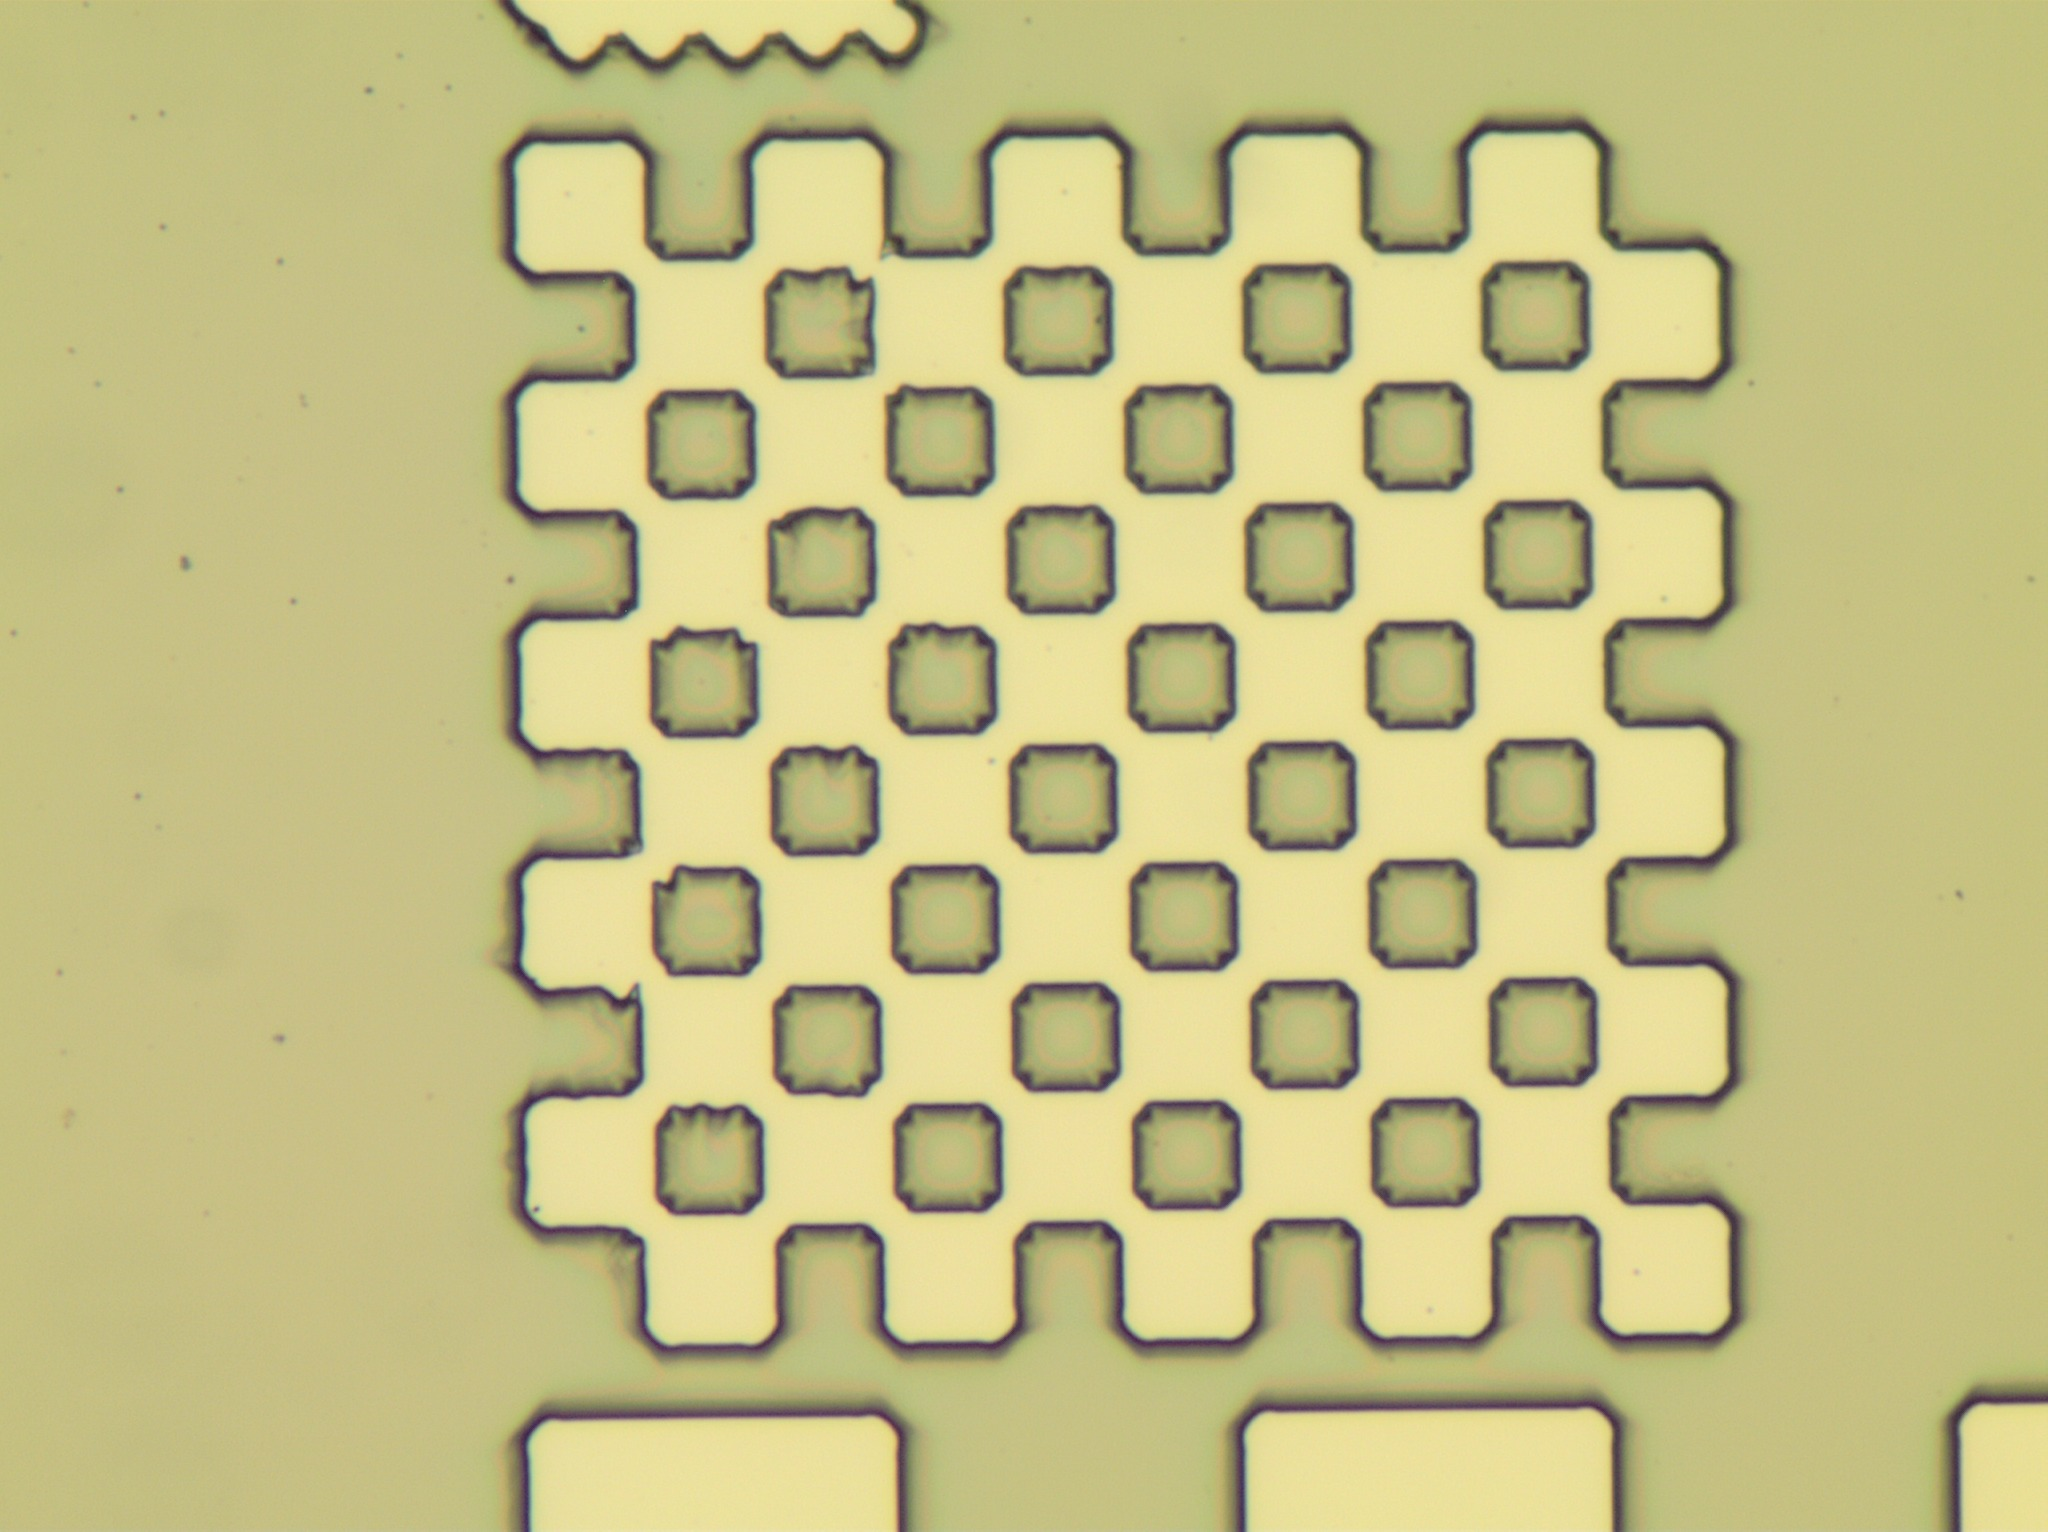
\includegraphics{data/b3f1.jpg}}
%  	\caption{b3f1}
%  	\label{fig:b3f1}
% \end{subfigure}
%  \end{figure*}








% % \todo[inline]{SEM}
% \begin{figure*}[!t]	
%     \centering
%     \begin{subfigure}[t]{0.24\linewidth}
%  	\centering
%  	\resizebox{\linewidth}{!}{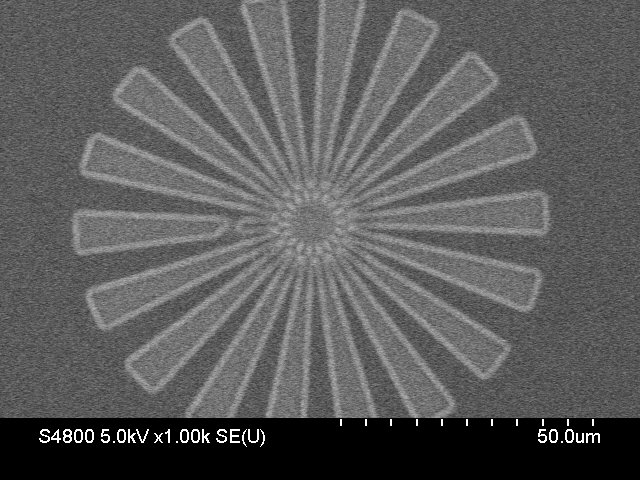
\includegraphics{data/sem/b3a1_q01.jpg}}
%  	\caption{SEM}
%  	\label{fig:b2d1_q1}
%  \end{subfigure}
% \hfill
%     \begin{subfigure}[t]{0.24\linewidth}
%  	\centering
%  	\resizebox{\linewidth}{!}{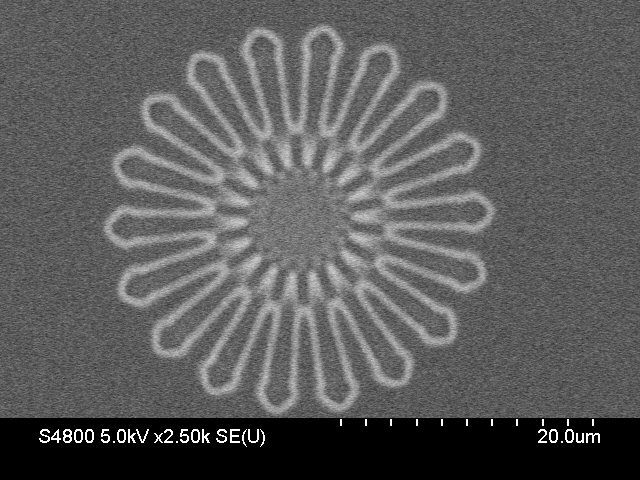
\includegraphics{data/sem/b3a2_q02.jpg}}
%  	\caption{SEM}
%  	\label{fig:b2d2_q2}
%  \end{subfigure}
% \hfill
%     \begin{subfigure}[t]{0.24\linewidth}
%  	\centering
%  	\resizebox{\linewidth}{!}{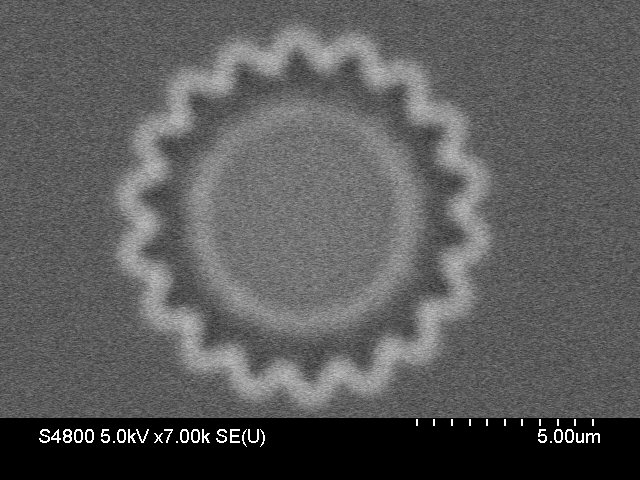
\includegraphics{data/sem/b3a3_q03.jpg}}
%  	\caption{SEM}
%  	\label{fig:b2d3_q3}
%  \end{subfigure}
% \hfill
%     \begin{subfigure}[t]{0.24\linewidth}
%  	\centering
%  	\resizebox{\linewidth}{!}{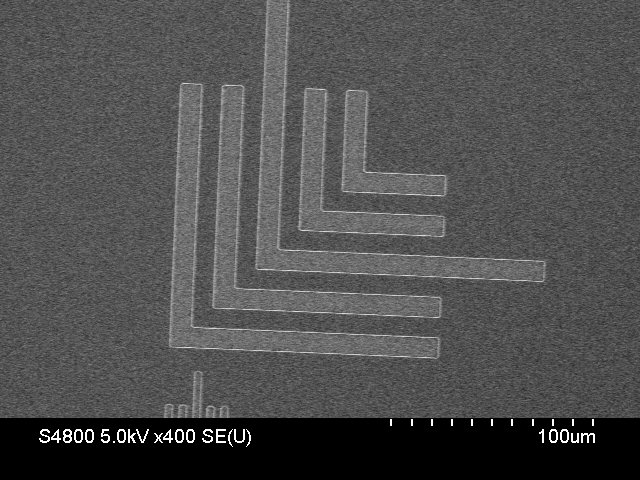
\includegraphics{data/sem/b3a11_q12.jpg}}
%  	\caption{SEM}
%  	\label{fig:b2d12_q12}
%  \end{subfigure}
% \end{figure*}

% \begin{figure*}[!t]	
%     \centering
%     \begin{subfigure}[t]{0.24\linewidth}
%  	\centering
%  	\resizebox{\linewidth}{!}{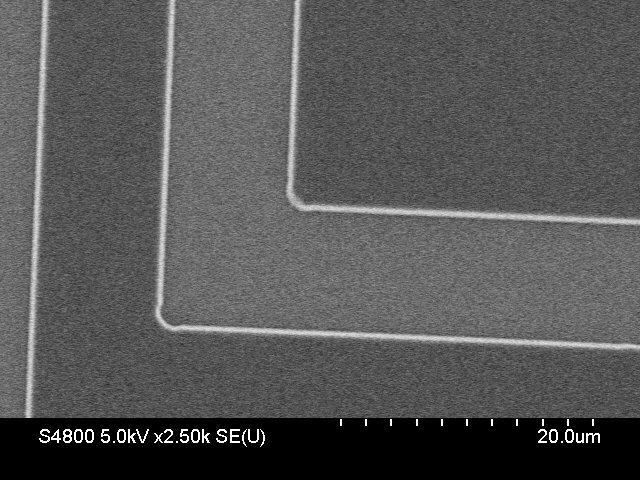
\includegraphics{data/sem/b3a11_q13.jpg}}
%  	\caption{SEM}
%  	\label{fig:b2d13_q13}
%  \end{subfigure}
% %\hfill
% %    \begin{subfigure}[t]{0.24\linewidth}
% % 	\centering
% % 	\resizebox{\linewidth}{!}{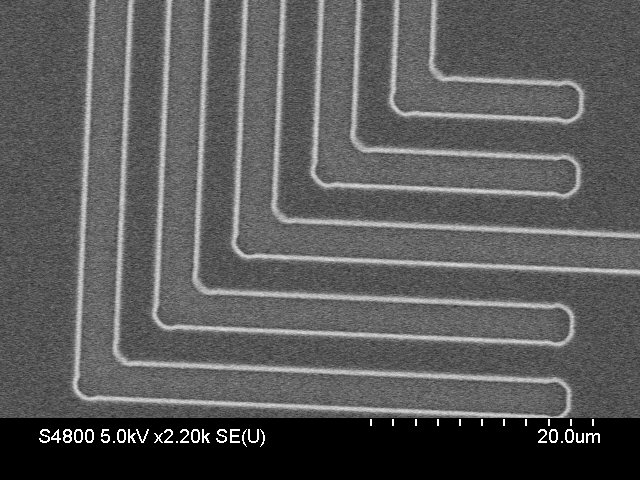
\includegraphics{data/sem/b3a11_q14.jpg}}
% % 	\caption{SEM}
% % 	\label{fig:b2d14_q14}
% %  \end{subfigure}
% \hfill
%     \begin{subfigure}[t]{0.24\linewidth}
%  	\centering
%  	\resizebox{\linewidth}{!}{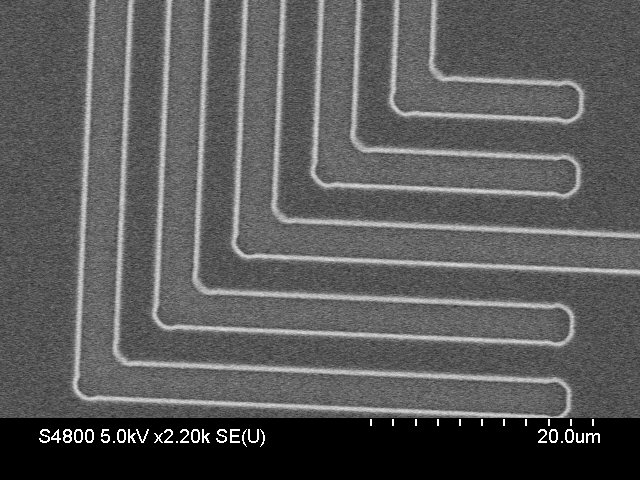
\includegraphics{data/sem/b3a11_q15.jpg}}
%  	\caption{SEM}
%  	\label{fig:b2d15_q15}
%   \end{subfigure}
% \hfill
%     \begin{subfigure}[t]{0.24\linewidth}
%  	\centering
%  	\resizebox{\linewidth}{!}{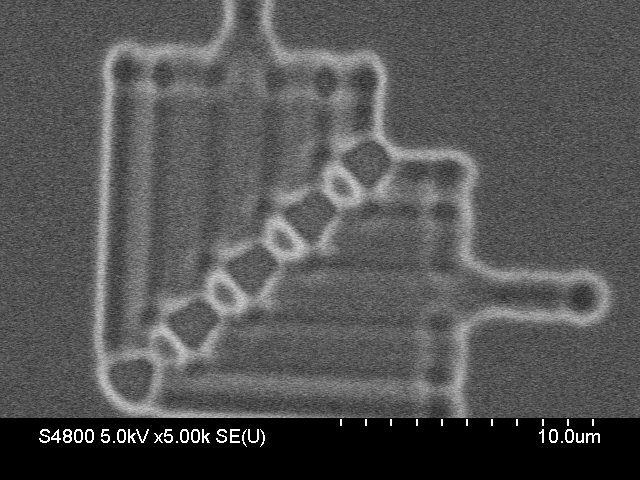
\includegraphics{data/sem/b3a11_q16.jpg}}
%  	\caption{SEM}
%  	\label{fig:b2d16_q16}
%  \end{subfigure}
% \end{figure*}
% \begin{figure*}[!t]	
%     \centering
%     \begin{subfigure}[t]{0.24\linewidth}
%  	\centering
%  	\resizebox{\linewidth}{!}{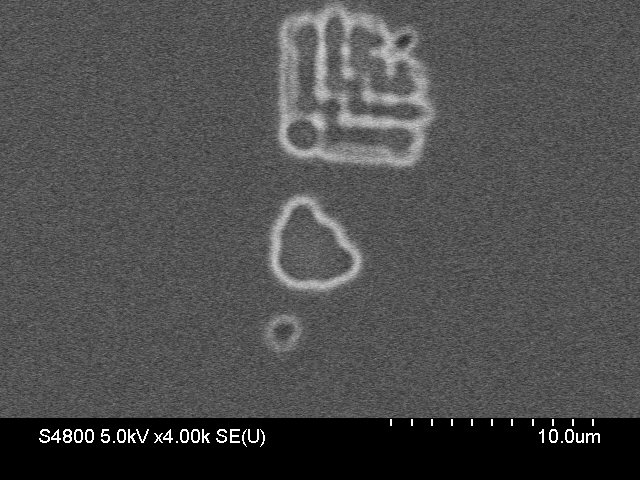
\includegraphics{data/sem/b3a11_q17.jpg}}
%  	\caption{SEM}
%  	\label{fig:b2d17_q17}
%  \end{subfigure}
% \hfill
% %    \begin{subfigure}[t]{0.24\linewidth}
% % 	\centering
% % 	\resizebox{\linewidth}{!}{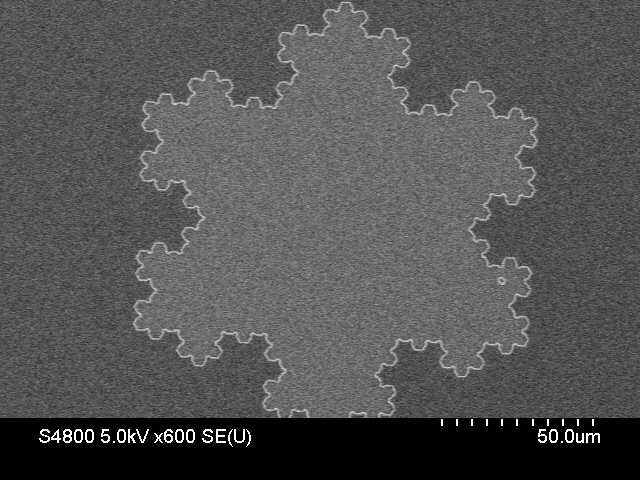
\includegraphics{data/sem/b3a11_q18.jpg}}
% % 	\caption{SEM}
% % 	\label{fig:b2d18_q18}
% % \end{subfigure}
% %\hfill
%     \begin{subfigure}[t]{0.24\linewidth}
%  	\centering
%  	\resizebox{\linewidth}{!}{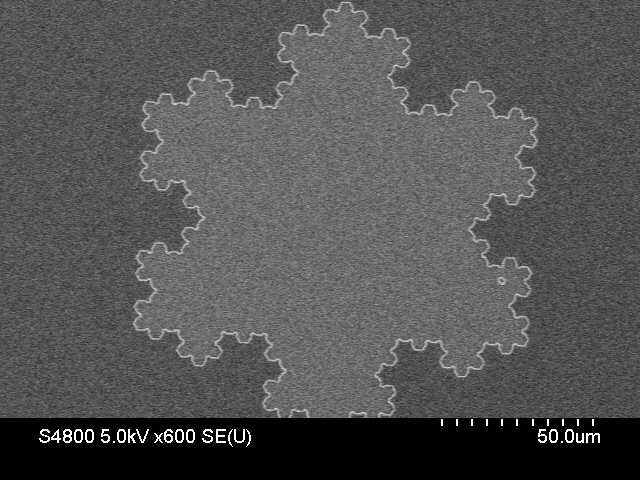
\includegraphics{data/sem/b3a11_q19.jpg}}
%  	\caption{SEM}
%  	\label{fig:b2d19_q19}
%  \end{subfigure}
% \hfill
%     \begin{subfigure}[t]{0.24\linewidth}
%  	\centering
%  	\resizebox{\linewidth}{!}{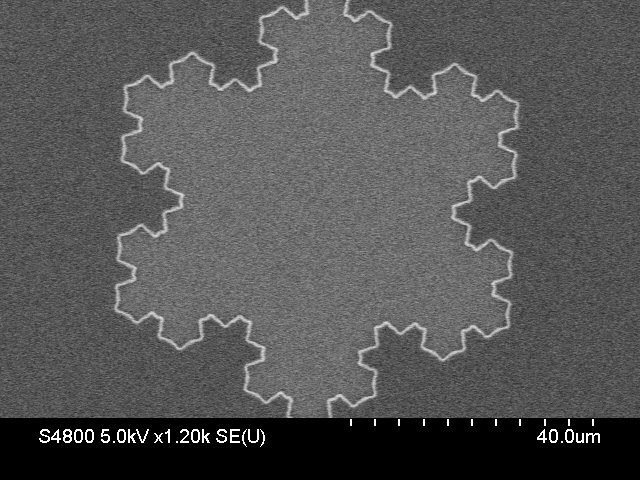
\includegraphics{data/sem/b3a11_q20.jpg}}
%  	\caption{SEM}
%  	\label{fig:b2d20_q20}
%  \end{subfigure}
% \end{figure*}


% \begin{figure*}[!t]	
%     \centering
%     \begin{subfigure}[t]{0.24\linewidth}
%  	\resizebox{\linewidth}{!}{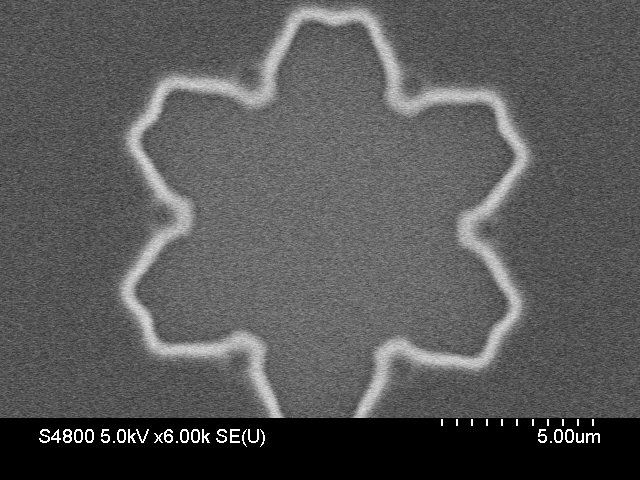
\includegraphics{data/sem/b3a11_q21.jpg}}
%  	\caption{SEM}
%  	\label{fig:b2d21_q21}
%  \end{subfigure}
% \hfill
%     \begin{subfigure}[t]{0.24\linewidth}
%  	\centering
%  	\resizebox{\linewidth}{!}{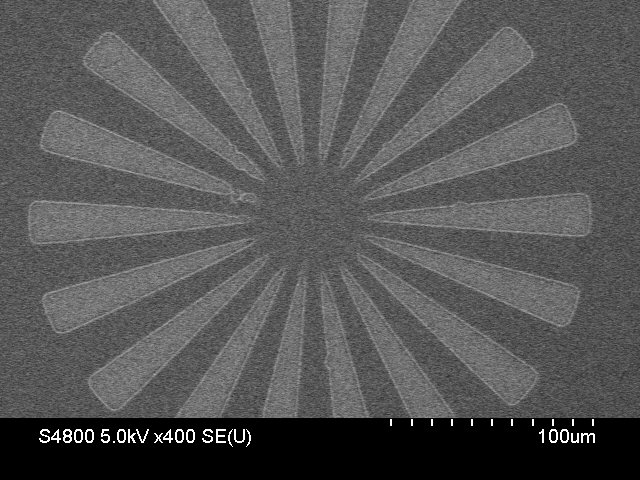
\includegraphics{data/sem/b2d22_q22.jpg}}
%  	\caption{SEM}
%  	\label{fig:b2d22_q22}
%  \end{subfigure}
% \hfill
%     \begin{subfigure}[t]{0.24\linewidth}
%  	\centering
%  	\resizebox{\linewidth}{!}{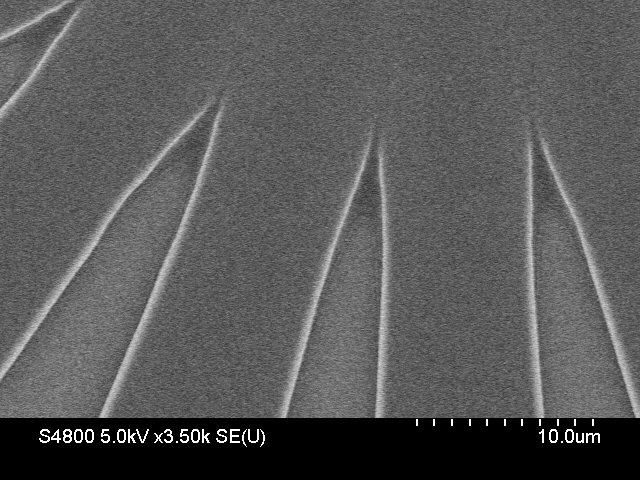
\includegraphics{data/sem/b2d23_q23.jpg}}
%  	\caption{SEM}
%  	\label{fig:b2d23_q23}
%  \end{subfigure}
% \hfill
%     \begin{subfigure}[t]{0.24\linewidth}
%  	\centering
%  	\resizebox{\linewidth}{!}{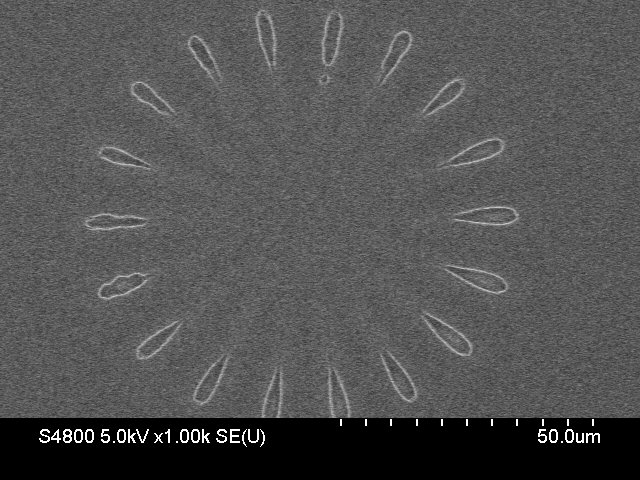
\includegraphics{data/sem/b2d24_q24.jpg}}
%  	\caption{SEM}
%  	\label{fig:b2d24_q24}
%  \end{subfigure}
% \end{figure*}

% \begin{figure*}[!t]	
%     \centering
%     \begin{subfigure}[t]{0.24\linewidth}
%  	\resizebox{\linewidth}{!}{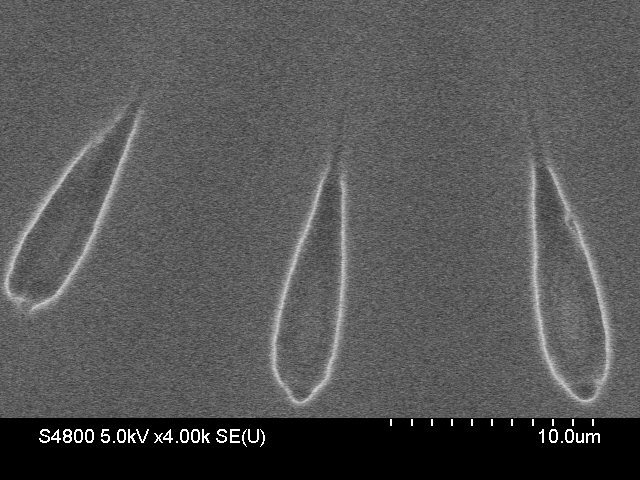
\includegraphics{data/sem/b2d25_q25.jpg}}
%  	\caption{SEM}
%  	\label{fig:b2d25_q25}
%  \end{subfigure}
% \hfill
%     \begin{subfigure}[t]{0.24\linewidth}
%  	\centering
%  	\resizebox{\linewidth}{!}{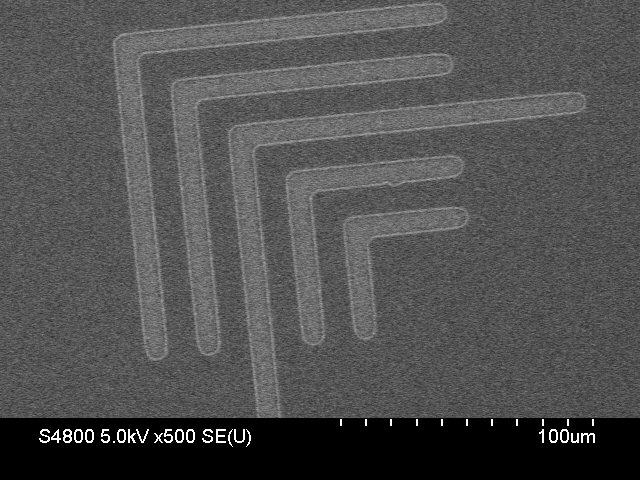
\includegraphics{data/sem/b2d30_q30.jpg}}
%  	\caption{SEM}
%  	\label{fig:b2d30_q30}
%  \end{subfigure}
% \hfill
%     \begin{subfigure}[t]{0.24\linewidth}
%  	\centering
%  	\resizebox{\linewidth}{!}{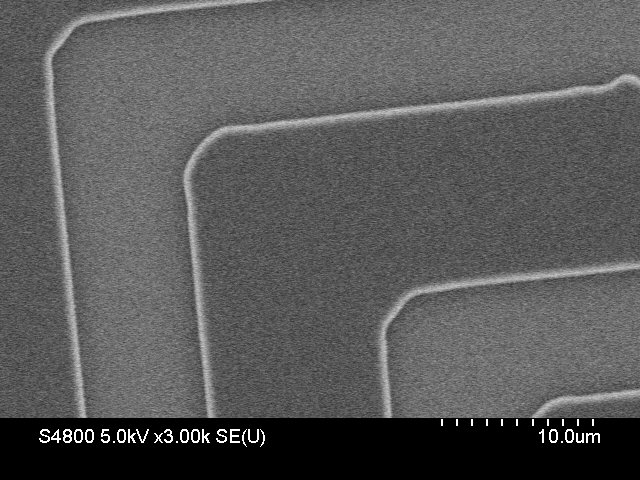
\includegraphics{data/sem/b2d31_q31.jpg}}
%  	\caption{SEM}
%  	\label{fig:b2d31_q31}
%  \end{subfigure}
% \hfill
%     \begin{subfigure}[t]{0.24\linewidth}
%  	\centering
%  	\resizebox{\linewidth}{!}{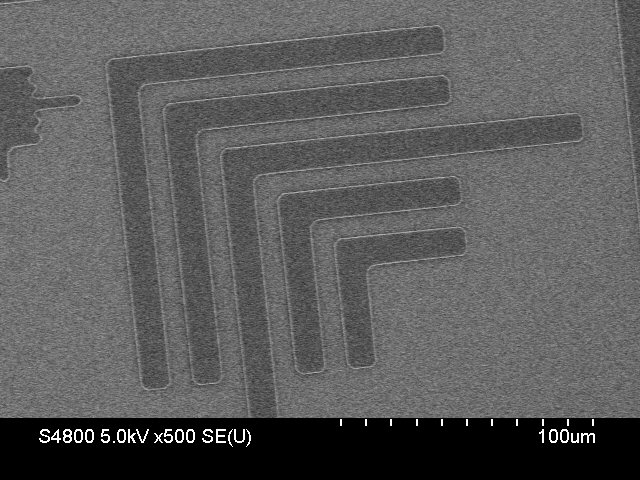
\includegraphics{data/sem/b2d31_q32.jpg}}
%  	\caption{SEM}
%  	\label{fig:b2d31_q32}
%  \end{subfigure}
% \end{figure*}



% \begin{figure*}[!t]	
%     \centering
%     \begin{subfigure}[t]{0.24\linewidth}
%  	\resizebox{\linewidth}{!}{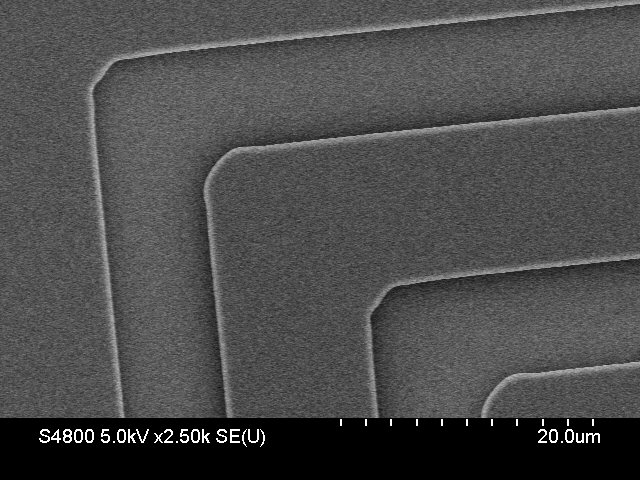
\includegraphics{data/sem/b2d33_q33.jpg}}
%  	\caption{SEM}
%  	\label{fig:b2d33_q33}
% \end{subfigure}
% \hfill
%     \begin{subfigure}[t]{0.24\linewidth}
%  	\centering
%  	\resizebox{\linewidth}{!}{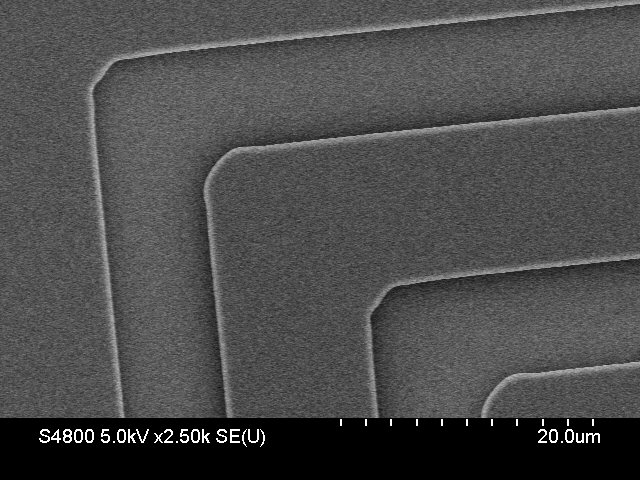
\includegraphics{data/sem/b2d33_q34.jpg}}
%  	\caption{SEM}
%  	\label{fig:b2d33_q34}
% \end{subfigure}
% \hfill
%     \begin{subfigure}[t]{0.24\linewidth}
%  	\centering
%  	\resizebox{\linewidth}{!}{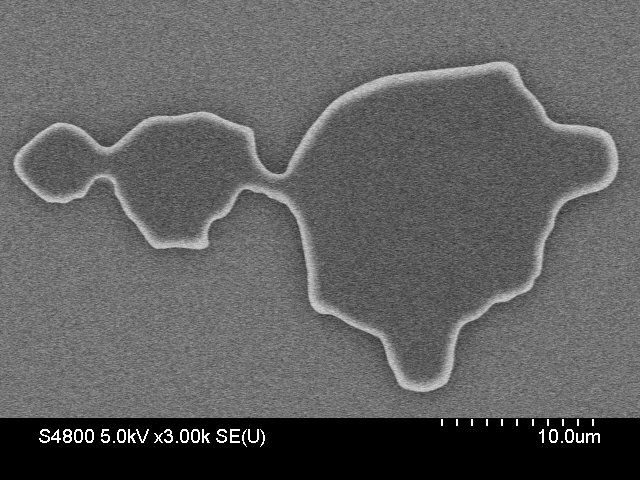
\includegraphics{data/sem/b2d33_q35.jpg}}
%  	\caption{SEM}
%  	\label{fig:b2d33_q35}
% \end{subfigure}
% \hfill
%     \begin{subfigure}[t]{0.24\linewidth}
%  	\centering
%  	\resizebox{\linewidth}{!}{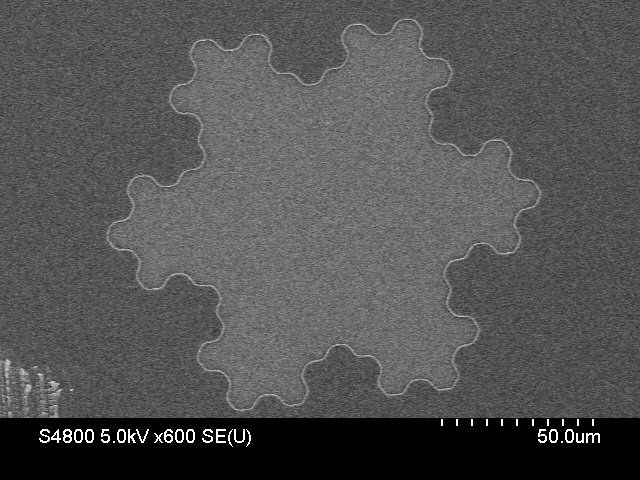
\includegraphics{data/sem/b2d36_q36.jpg}}
%  	\caption{SEM}
%  	\label{fig:b2d36_q36}
% \end{subfigure}
%  \end{figure*}
% \begin{figure*}[!t]	
%     \centering
%     \begin{subfigure}[t]{0.24\linewidth}
%  	\resizebox{\linewidth}{!}{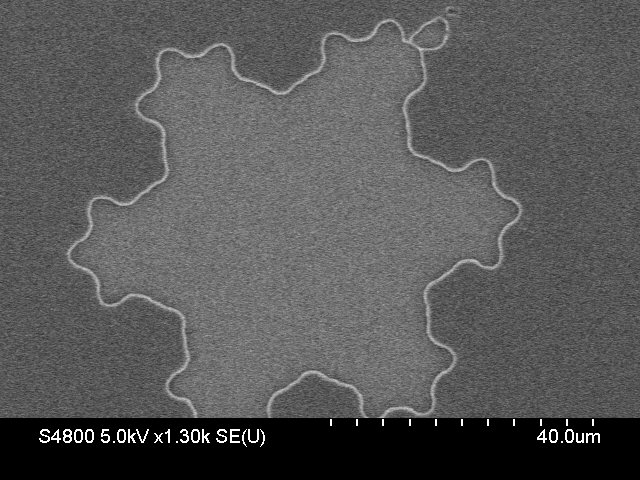
\includegraphics{data/sem/b2d36_q37.jpg}}
%  	\caption{SEM}
%  	\label{fig:b2d36_q37}
% \end{subfigure}
% \hfill
%     \begin{subfigure}[t]{0.24\linewidth}
%  	\centering
%  	\resizebox{\linewidth}{!}{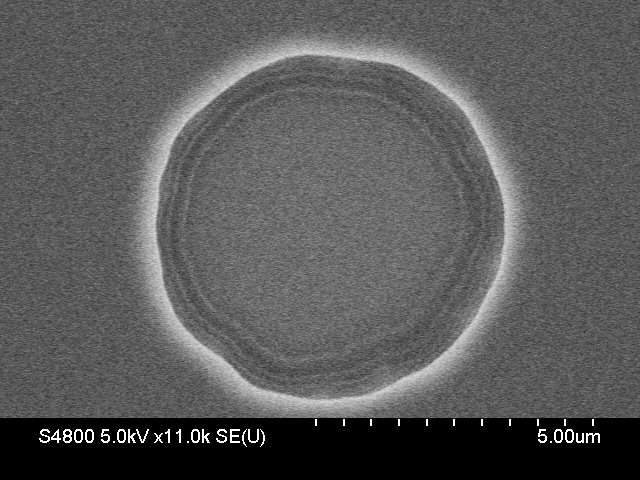
\includegraphics{data/sem/b2d38_q38.jpg}}
%  	\caption{SEM}
%  	\label{fig:b2d38_q38}
% \end{subfigure}
% \hfill
%     \begin{subfigure}[t]{0.24\linewidth}
%  	\centering
%  	\resizebox{\linewidth}{!}{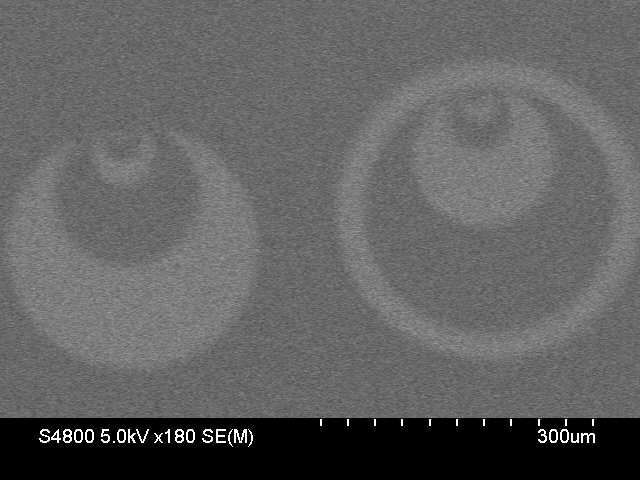
\includegraphics{data/sem/b2d39_q39.jpg}}
%  	\caption{SEM}
%  	\label{fig:b2d39_q39}
% \end{subfigure}
% \hfill
%     \begin{subfigure}[t]{0.24\linewidth}
%  	\centering
%  	\resizebox{\linewidth}{!}{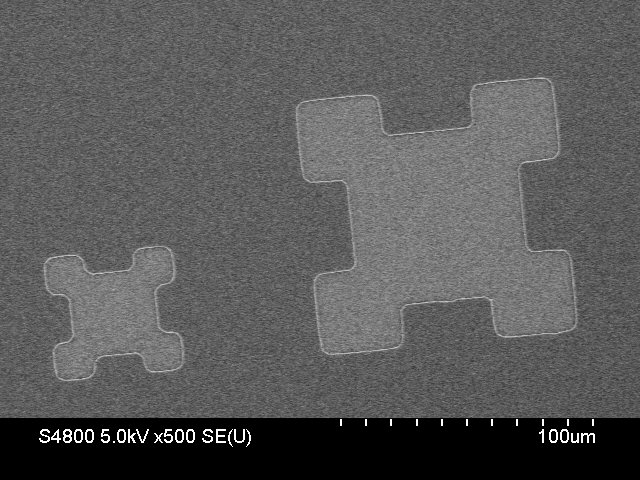
\includegraphics{data/sem/b2d40_q40.jpg}}
%  	\caption{SEM}
%  	\label{fig:b2d40_q40}
% \end{subfigure}
%  \end{figure*}

%  \begin{figure}[!t]
%  	\centering
%  	\resizebox{\linewidth}{!}{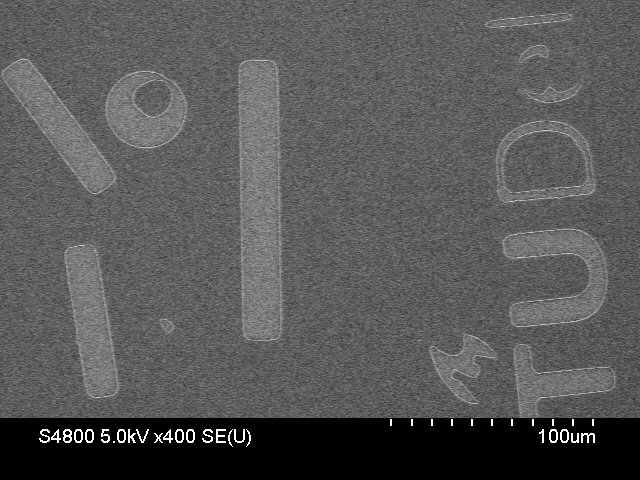
\includegraphics{data/sem/b2d41_q41.jpg}}
%  	\caption{SEM}
%  	\label{fig:b2d41_q41}
%  \end{figure}
% %
% %\begin{figure*}[!t]	
% %    \centering
% %    \begin{subfigure}[t]{0.24\linewidth}
% %	\resizebox{\linewidth}{!}{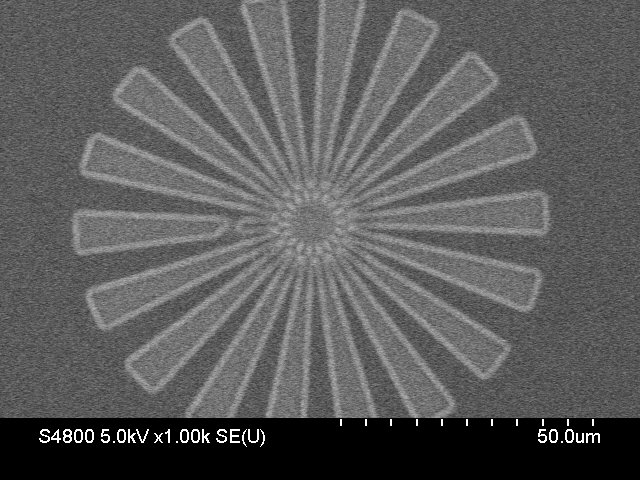
\includegraphics{data/sem/b3a1_q01.jpg}}
% %	\caption{SEM}
% %	\label{fig:b2d1_q1}
% %\end{subfigure}
% %\hfill
% %    \begin{subfigure}[t]{0.24\linewidth}
% %	\centering
% %	\resizebox{\linewidth}{!}{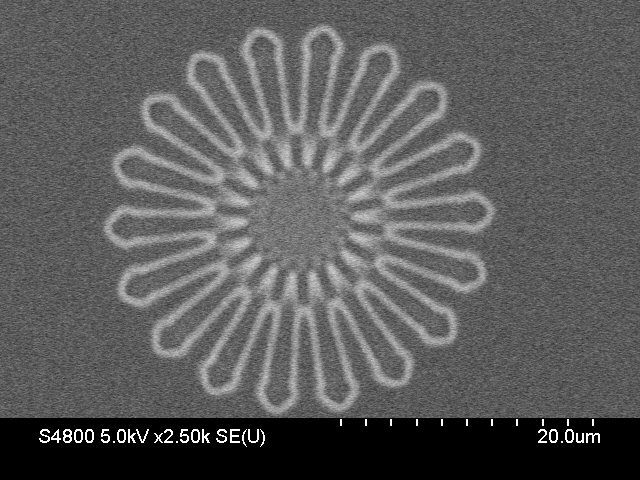
\includegraphics{data/sem/b3a2_q02.jpg}}
% %	\caption{SEM}
% %	\label{fig:b2d2_q2}
% %\end{subfigure}
% %\hfill
% %    \begin{subfigure}[t]{0.24\linewidth}
% %	\centering
% %	\resizebox{\linewidth}{!}{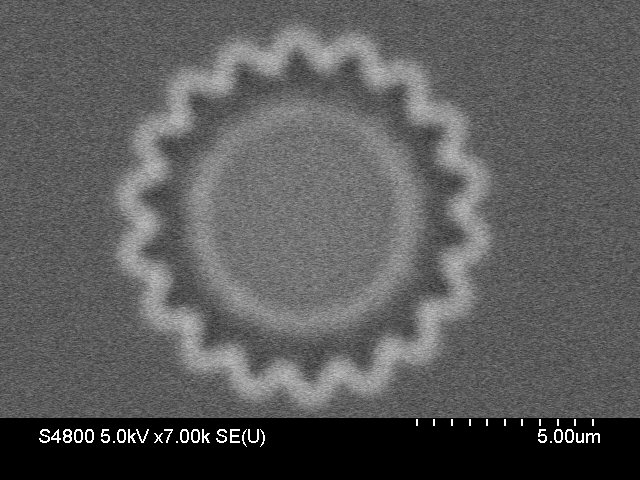
\includegraphics{data/sem/b3a3_q03.jpg}}
% %	\caption{SEM}
% %	\label{fig:b2d3_q3}
% %\end{subfigure}
% %    \begin{subfigure}[t]{0.24\linewidth}
% %	\centering
% %	\resizebox{\linewidth}{!}{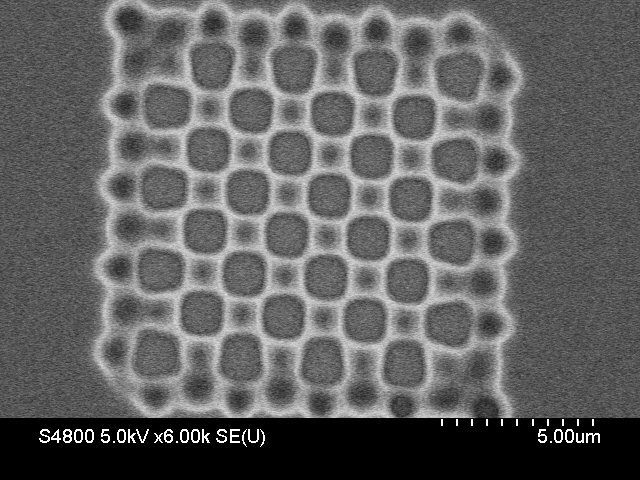
\includegraphics{data/sem/b3a10_q10.jpg}}
% %	\caption{SEM}
% %	\label{fig:b2d10_q10}
% %\end{subfigure}
% %\end{figure*}

% \begin{figure*}[!t]
% \centering
%     \begin{subfigure}[t]{0.3\linewidth}
% 	\centering
% 	\resizebox{\linewidth}{!}{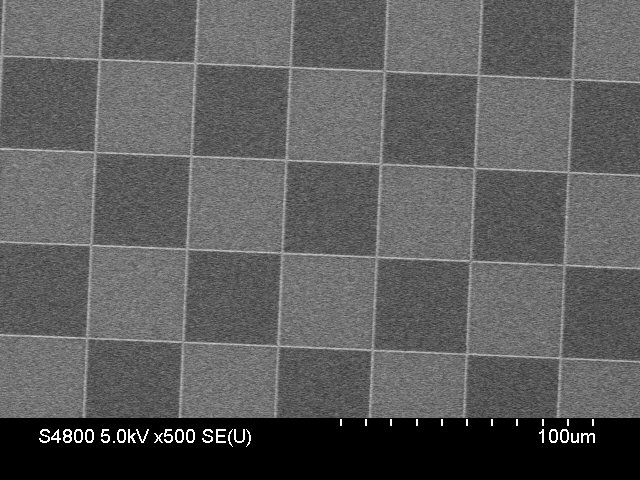
\includegraphics{data/sem/b3a4_q04.jpg}}
% 	\caption{Structure size of $\sim$32 $\mu$m.}
% 	\label{fig:b2d4_q4}
% \end{subfigure}
% \hfill
%     \begin{subfigure}[t]{0.3\linewidth}
% 	\centering
% 	\resizebox{\linewidth}{!}{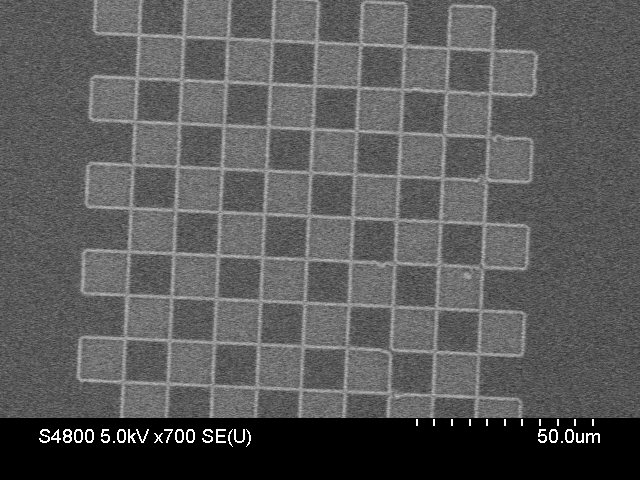
\includegraphics{data/sem/b3a6_q06.jpg}}
% 	\caption{Structure size of $\sim$10 $\mu$m.}
% 	\label{fig:b2d6_q6}
% \end{subfigure}
% \hfill
%     \begin{subfigure}[t]{0.3\linewidth}
% 	\centering
% 	\resizebox{\linewidth}{!}{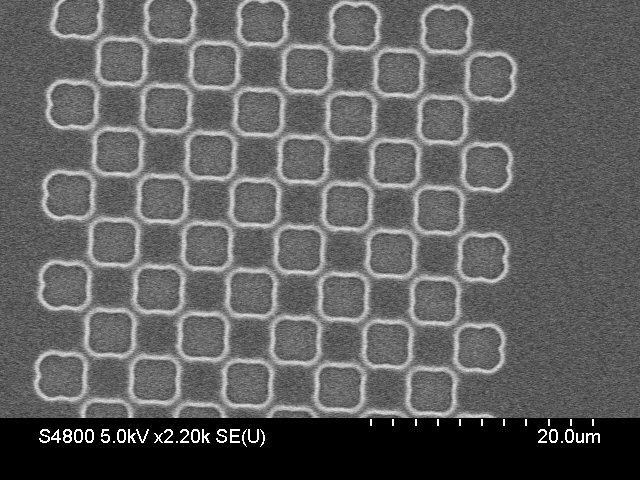
\includegraphics{data/sem/b3a8_q08.jpg}}
% 	\caption{Structure size of $\sim$3 $\mu$m.}
% 	\label{fig:b2d8_q8}
% \end{subfigure}
% \end{figure*}
